% -*- root: These.tex -*-
\graphicspath{{FigureIntroduction/}}

\chapter*{Introduction}

\epigraph{Nous sommes comme un patient qui sort d'un coma aussi long que la vie d'une étoile.
Ce dont nous ne pouvons nous souvenir, nous devons le redécouvrir }{---  \textup{Robert Charles Wilson}  Axis}

\epigraph {L'humanité se compose de plus de morts que de vivants } { --- \textup{Auguste Comte}}

% Citer quelque part l'edito de Denise Pumain ! 

La géographie est partie prenante des bouleversements considérables introduits par la numérisation dans l’ensemble des pratiques scientifiques depuis à peine deux décennies, et cela à plusieurs titres. Les manifestations les plus évidentes tiennent à la prolifération des informations individuelles \enquote{géolocalisées} désormais disponibles sur toutes sortes de support, et notamment, ce qui est entièrement nouveau, en situations de mobilité \autocite{FenChong2012}. Les dispositifs techniques de repérage comme le GPS et l’ouverture des systèmes d’information géographique à l’interactivité grâce à la version 2.0 d’Internet donnent lieu au développement d’une \enquote{géographie volontaire} \autocite{Goodchild2007}, qui conduit à diffuser auprès du grand public des pratiques et des savoir-faire jusqu’ici réservés aux professionnels. Le très grand nombre des institutions privées ou publiques qui partagent ce nouvel engouement pour l’inscription spatiale de leurs activités, tout comme la croissance fabuleuse des \enquote{ réseaux sociaux } sur Internet  contribuent à l’immense développement de ce qu’il est convenu d’appeler, sans traduction en français, les \enquote{ big data }. Ces masses de données très labiles, évoluant souvent en temps réel, qu’il est relativement facile de collecter à différents niveaux d’agrégation, posent de nouveaux défis aux géographes en termes de traitement des ces informations, tout autant qualitatives que quantitatives. 

Les méthodes classiques de résumé des connaissances par la modélisation et la visualisation doivent être considérablement transformées pour s’adapter à cette nouvelle donne. Mais il serait dommageable de ne pas appuyer notre réflexion sur les pratiques passées pour dessiner un horizon des transformations à venir. Avant d’en arriver au propos de cette thèse, il nous semble indispensable d’opérer un retour sur les expériences de modélisation qui ont été conduites depuis plus de soixante ans dans le cadre paradigmatique général de la systémique. Notre sujet de thèse et notre hypothèse de recherche principale (présentée ci-dessous page 17), s’inscrivent en effet dans une longue histoire collective dont il nous faut repérer les forces et les faiblesses afin de justifier la démarche que nous avons adoptée. 

En effet, l'accumulation et l'exploitation de données est une problématique récurrente pour les géographes et les sciences humaines en général, cela depuis les années 1950-60 \autocite{Kao1963, Hagerstrand1967b} \autocite[386]{Barnes2011} et les premières grandes récoltes de données informatisées sur la population. On pourra citer à ce propos \textcite{Gullahorn1966} lorsqu'il pointe l'importance pour les sciences humaines et sociales du recueil \textit{Computer methods in the analysis of large-scale social systems} qui retrace les discussions issues d'un des tout premiers grands rassemblements inter-disciplinaires organisés par le MIT. Cette conférence piloté par un sociologue de la section \enquote{Urban Studies} du MIT \autocite{Beshers1965} propose de faire le point sur les nouvelles méthodologies et techniques quantitatives et leur utilisations dans les différentes disciplines en science sociales, avec cette volonté marqué de reprendre le contrôle sur la construction des modèles, \footnote{Un point de vue parmis les nombreux dans ce livre, celui de l'éditeur \textcite[194]{Beshers1965} : \foreignquote{english}{The development of a simulation model must by by persons intimately familiar with the subject matter. This principle has been violated in the past by excessive delegation of resposability to mathematicians and programmers interested primarly in questions of structure and style.} }  afin de faire face au \textit{Big Data} de l'époque, les données américaines de recensement \textit{U.S Census}. Une question brûlante d'actualités à l'ère du \textit{Big data}, car 50 ans plus tard, et des centaines d'innovations techniques plus tard, peut on enfin dire que les scientifiques ont pris le plein contrôle de leur données et des outils associés permettant la construction des modèles ?

\begin{figure}[!h]
\begin{sidecaption}[fortoc]{Le \enquote{champignon informationnel} proposé par Frédéric Kaplan est révélateur de l'augmentation du champ d'expérimentation rendu possible par la numérisation des données, puis la simulation numérique.}[fig:I_Champi]
 \centering
 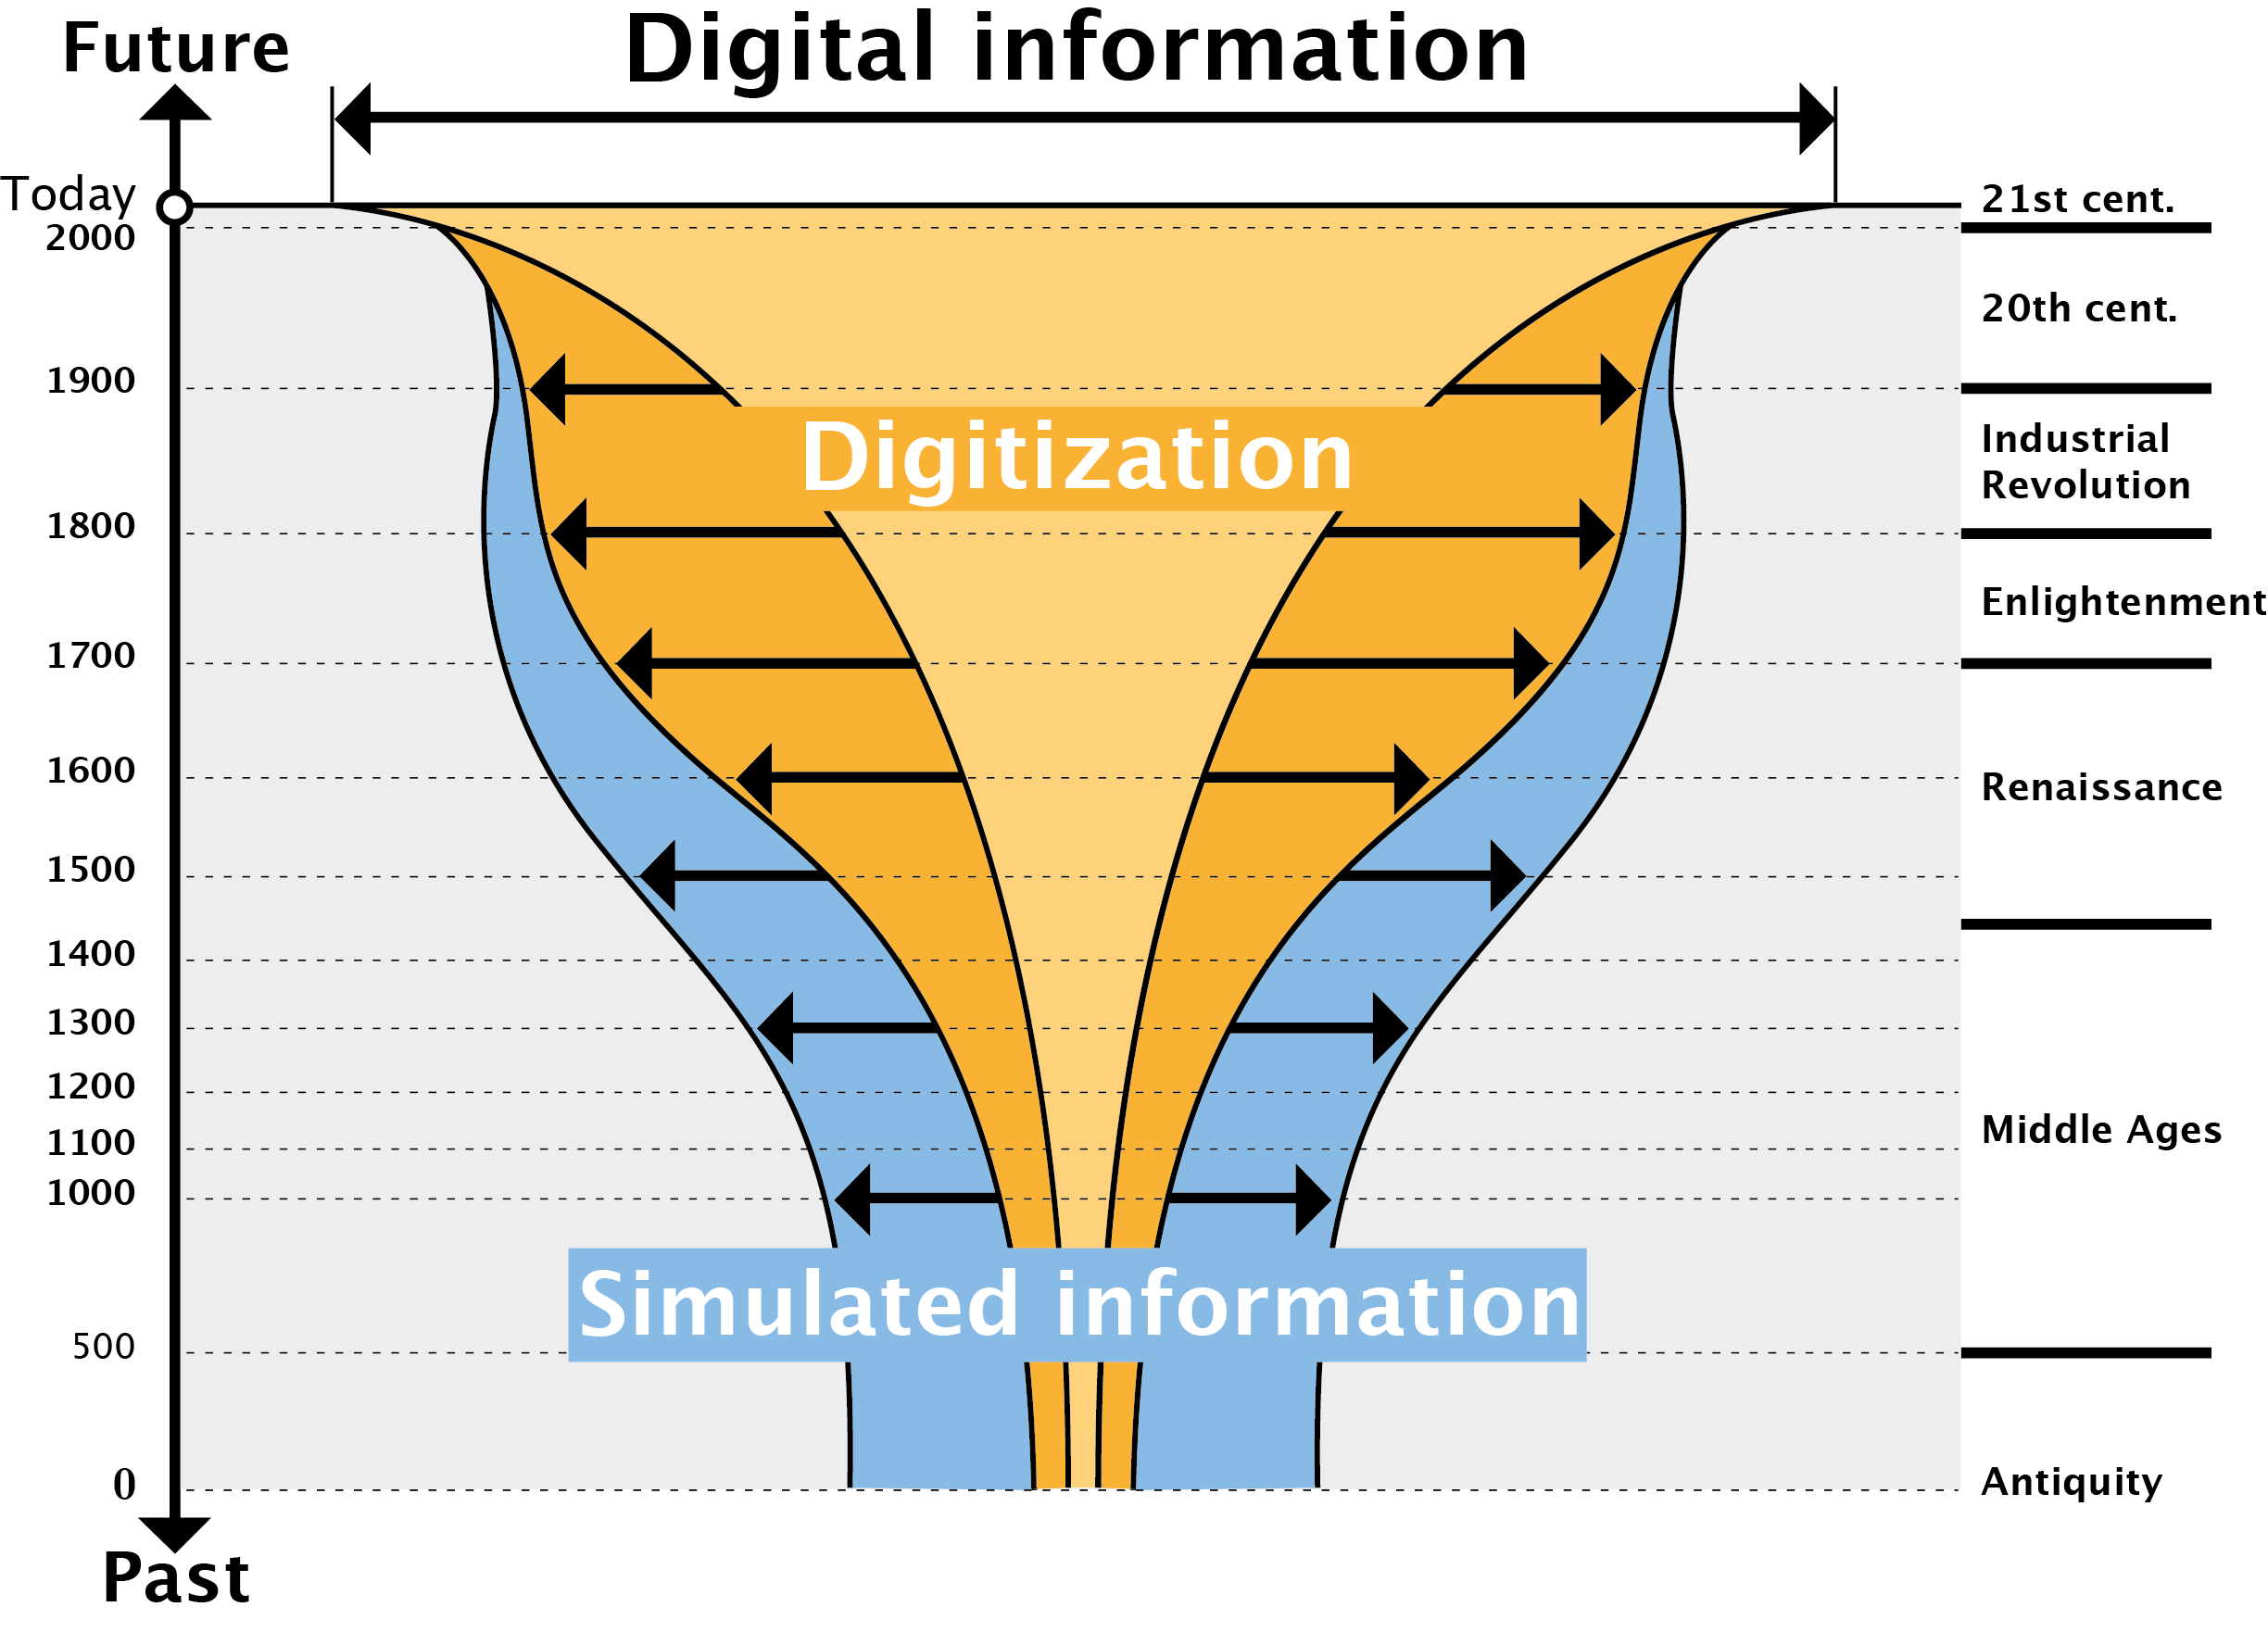
\includegraphics[width=\linewidth]{champignonKaplan.png}
 \legend{Legendary table}
  \end{sidecaption}
\end{figure}

Mais cela serait une erreur que de limiter l'application de ces nouveaux outils aux seuls stockages numériques récents, et ne pas citer l'importance du volume de connaissances collectionnées ces derniers siècles par certaines sciences sociales telles que l'archéologie ou encore la géographie. Des données qui n'attendent qu'à être cataloguées numériquement puis explorées dans le but d'en faire ressortir de nouveaux motifs. Voir la figure \ref{fig:I_Champi} \footnote{Voir l'article sur son blog \href{http://fkaplan.wordpress.com/2013/03/14/lancement-de-la-venice-time-machine/}{@FrédéricKaplan}}

%\begin{figure}[tb]
%\raggedright
%\begin{sidecaption}{This is a subcaption just for illustration purposes. This is a subcaption just for illustration purposes. 
%Champignon Informationnel de Frédéric Kaplan. Page number is \LARGE\textbf{\thepage}}[fig:test]
%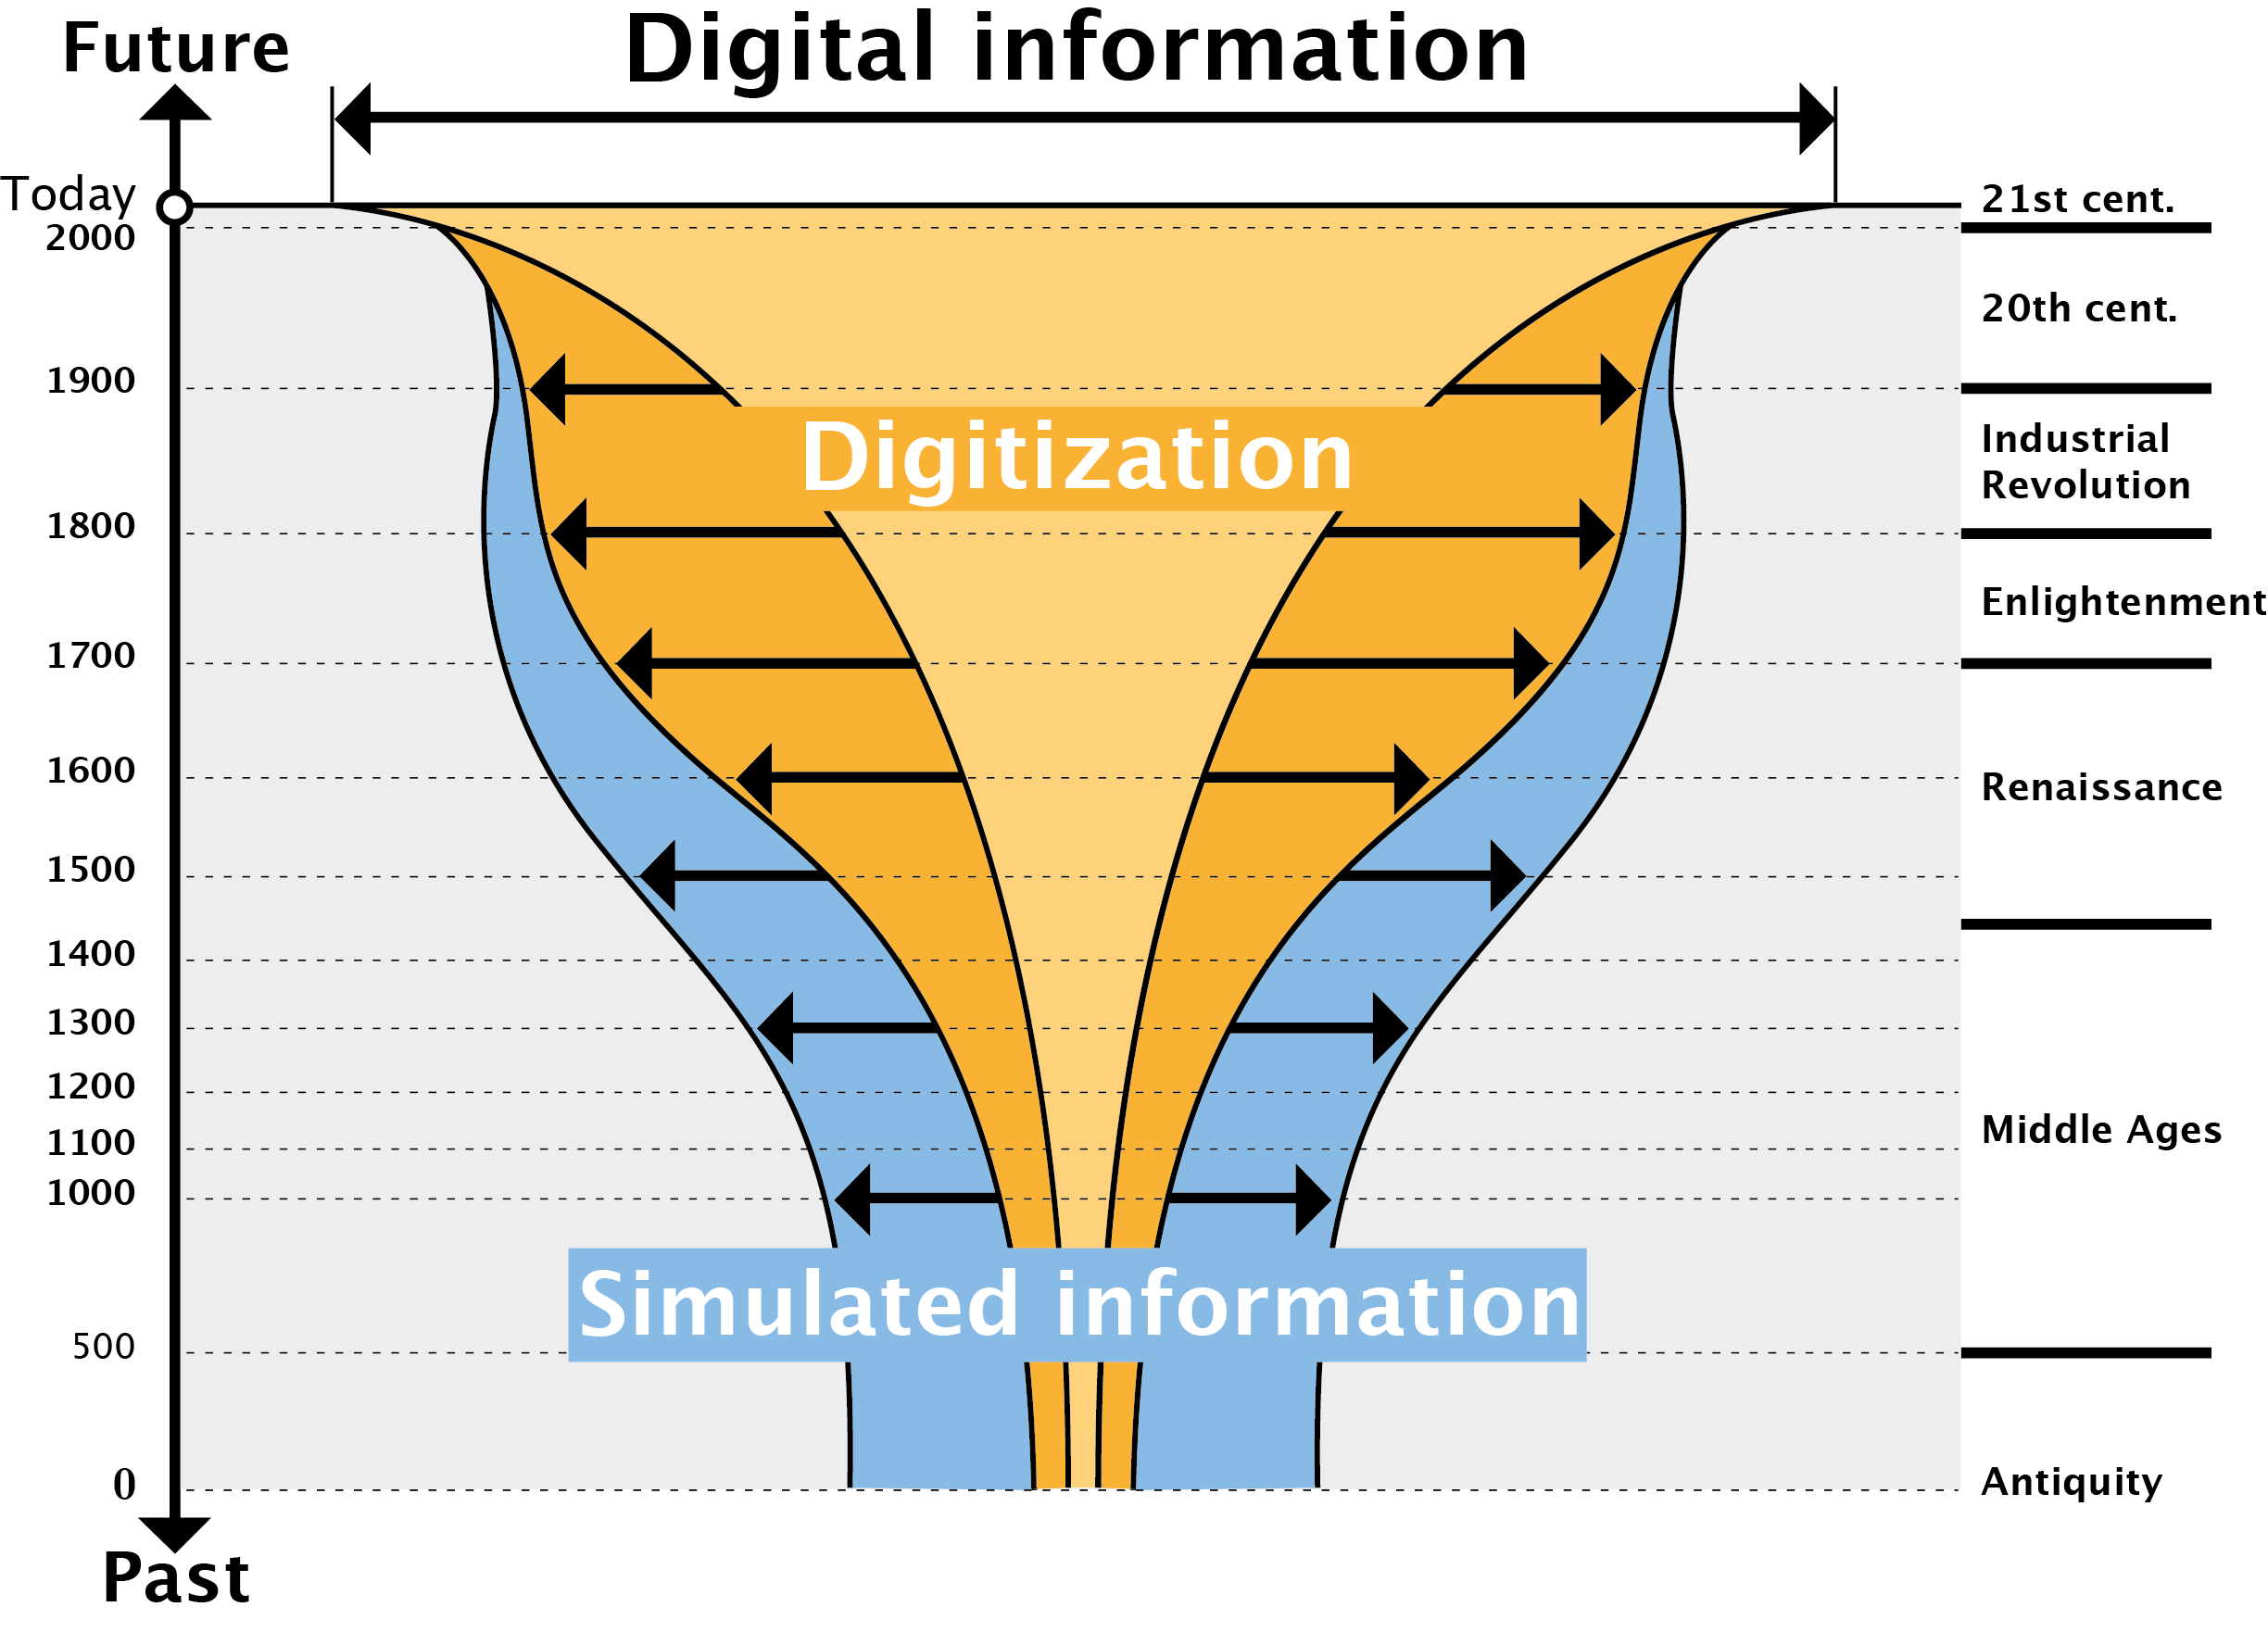
\includegraphics[width=\linewidth]{champignonKaplan.png}
%\end{sidecaption}
%\end{figure}

La classification automatique des données par l'ordinateur mais aussi la construction de modèles et leur simulation (au sens d'abord mathématique et parfois algorithmique du terme) apparaît rapidement comme un enjeux pour la géographie. La simulation de ces derniers apparaissant comme un outil de construction de connaissance absolument naturel et nécessaire pour confronter et construire les théories en rapport avec ces données \autocite{Kao1963, Hagerstrand1967b}. L'image de cette communauté inter-disciplinaire agitant et confrontant ses problématiques méthodologiques, techniques, théoriques dans un but de progression commun, fait écho à des revendications plus récente \footnote{On pensera notamment à la communauté ABM inter-disciplinaire qui gravite autour de la revue JASSS fondée en  1990}. En réalité cet esprit de partage tient d'une \enquote{volonté commune} qui apparaît quasiment avec l'apparition et la démocratisation des techniques de simulation. C'est ainsi que l'on trouve trace des efforts de cette communauté de chercheurs dans plusieurs ouvrages tels que \autocite{Beshers1965,Naylor1966,Dutton1971,Guetzkow1962,Guetzkow1972}.

A ce sujet \textcite{Fleisher1965} produit une réflexion tout à fait remarquable par sa lucidité et son anticipation, comme en témoigne sa conclusion : \foreignquote{english}{I have argued that in the near future the social science will remain largely empirical and that simulation can serve as a device for making experiments \textbf{in vitro}. I think that this use is more important, at this time, than the massive making of models and that the principal contribution of simulation lies in the direction of intelligent, vivacious empiricism} \autocite{Fleisher1965}

%Forrester1969 a ce sujet "In the social sciences failure to understand systems is often blamed on inadequate data... The barrier is deficiency in the existing theory of structure." \autocite[355]{Batty1976}

\subsection{La simulation de modèles au cœur de la construction des connaissances en sciences sociales et en géographie}

La plupart des disciplines connaissent une phase de transformation après les années 1950-60 qui va de pair avec la découverte de nouvelles méthodes quantitatives et la volonté d'opérer un rapprochement avec les techniques scientifiques de construction des connaissances communes aux sciences naturelles.

L'apparition et la diffusion de ces techniques quantitative n'est pas le résultat d'une convergence unique, mais bien d'une succession de moments dont la fréquence et l'étalement temporel est difficile à cerner et empêche sur ce sujet toute exhaustivité. 

On retiendra toutefois plusieurs grands facteurs, dont certains qui peuvent paraître étonnamment antinomiques. Une convergence qui s'illustre dans la richesse et la diversité des transformations qui touche la discipline géographique entre 1950 et 1970, un constat déjà établi par bien d'autres auteurs \autocite{Varenne2014} :

%Il manque l'écologie, cf unwin1992 121

\paragraph{L'influence de l'école néo-positiviste}

Pour les géographes, la première influence \footnote{Dont la portée initiale se limite surtout aux géographes ayant étudiés sur les bancs de l'université de Washington et d'Iowa \autocite[554]{Barnes2001a} \autocite[120-121]{Unwin1992}, ce qui ne change rien à l'importance des ouvrages écrits par ces mêmes géographes.} qui marque la fondation de cette \enquote{nouvelle géographie} est probablement à chercher dans les répercussions chez un certain nombre de géographes américains du programme néo-positiviste (Bergman, Hempel, etc.) et de ses critiques les plus proches (Popper), visant la reconstitution d'une unité des sciences au travers d'une mise en logique des énoncés d'observations. 

Le néo-positivisme est un courant philosophique nés à Vienne, dont une partie des membres est poussé à l'exode sous la pression du régime Nazi. L'installation d'une partie de ses membres aux états-unis, va se substituer au courant pragmatiste existant \footnote{Un changement qui amènent forcément à laisser quelques traces, un thème encore peu étudié en géographie jusqu'à présent. \textcite[123]{Wilson1995} affirme ainsi que les pragmatistes \foreignquote{english}{[...] had created the conditions in which logical positivism and other analytic philosophies could flourish and ultimately displace them as the dominant voice in mid-century philosophical debates} mais aussi les conditions de son dépassement \foreignquote{english}{Pragmatism, then, not only created the conditions in which logical positivism and analytic philosophy could flourish in the United States, it also contained the seeds of the postanalytic philosophies that have attempted to move beyond [...] } }, et va se diffuser à la fois sur les bancs des écoles, mais aussi via les grand instituts scientifique après guerre représentant de cette science \foreignquote{english}{mainstream}, organisés aux états-unis autour de l'ordinateur. La RAND fait partie de ses instituts fondé après guerre, qui approche dès 1947 les sciences sociales \autocite{Rand106}, et n'hésitent pas à mettre en avant par la suite les stars de la philosophie positiviste de l'époque comme Reichenbach. \autocite[384-385]{Barnes2011} 

Une vision de la science certes réductionniste mais qui fournit plus qu'une idéologie, une démarche scientifique inspirée des sciences naturelles, à savoir l'hypothético-déductivisme. Un programme qui moyennant quelques assouplissements sous la plume des théoriciens comme Bunge \autocite{Bunge1962}, Harvey \autocite{Harvey1969}, ou encore Olsson \autocite{Olsson1970}, fait tout à fait écho à cette volonté nomothétique et ce refus de l'exceptionalisme chez les géographes frondeurs des débuts.  

\paragraph{L'émergence d'une pensée holiste dans les sciences}

L'érosion d'un dogme dans les sciences naturelles; celui du déterminisme scientifique hérité de la pensée \enquote{classique} qui plonge de nombreuses disciplines en \enquote{crises} \autocite[20-23]{Pouvreau2013}. Une transition que l'on peut observer au travers de différents travaux majeurs, comme la statistique des lois de Boltzman pour la thermodynamique, ou le principe d’indétermination d'Heisenberg pour la mécanique quantique. Cette remise en cause peut également être associée à l'émergence d'une pensée \enquote{holiste} (ou pensée de la \enquote{totalité}) qui se construit en confrontation avec la pensée réductionniste historique.

\paragraph{L'apparition de mouvements inter-disciplinaires fédérateurs}

L'apparition de grands mouvements de convergence inter-disciplinaires dont certains prennent la forme de paradigme du fait de leur portée d'application  : Cybernétique de Wiener, \textit{projet} de la \foreignquote{english}{General System Theory} de Bertalanffy \autocite[9]{Pouvreau2013}, et d'autres remettent au gout du jour des écoles de pensées plus anciennes, comme celle de la \enquote{social physics} de Stewart \autocite{Stewart1947}. Par la suite et surement du fait des liens développés à l'université de Pennsylvanie, lieu de ses études, et siège de la fondation de la science régionale d'Isard en 1954, Stewart sera amené à publier dans la revue \textit{Regional Sciences} \autocite{Stewart1958}}.

Les retombées de ces interactions sur la géographie sont importantes \footnote{ A condition de ne pas oublier qu'une partie de ces concepts existent de façon sous-jacente aux disciplines, ce qui explique parfois leur rapidité d'acceptation. C'est le cas de l'approche systémique développé par la cybernétique quand elle ne fait pas qu'apposer un nom commun sur des concepts déjà étudiés, fait alors écho à des révolution méthodologiques en attente d'être activés. \textcite[5]{Batty1976} résume la situation ainsi \foreignquote{english}{The idea of systems being described in terms of structure and behaviour, in terms of input and output, and the notion of purposeful control of such systems in terms of negative and positive feedbacks, appeared to many social scientists an ideal description of their systems of interest and thus the approach has come to be used in more-or-less all of the social sciences}.}, et fournissent tout autant : (i) des concepts généraux en correspondances avec les débats qui anime l'ensemble des sciences : sensibilité aux conditions initiales, équifinalité, bifurcation et catastrophe, boite noire, rétro-causalité, hiérarchie d'emboitement, etc.) , (ii) un catalogue d'isomorphisme supplémentaire dont la correspondance reste à évaluer dans notre discipline \autocite{Wilson1969}, (iii)  une méthodologie et une typologie des modèles tirés de la recherche opérationnelle \autocite{Ackoff1962} \footnote{Une discipline proche du projet bertalanffien en bien des aspects} et largement revendiqués par les géographes dans la décennie 1960-70 \autocite{Kohn1970}, notamment  par les pionniers comme \autocite{Berry1964, Haggett1965}, (iv) la découverte d'une nouvelle science mathématique de la dynamique en correspondance avec ces nouveaux concepts, accessible soit par un vocabulaire graphique opérationnalisable \autocite{Forrester1961}, soit par des langage de programmation plus traditionnels ! On citera parmi les pionniers dans l'exploration de cette convergence en géographie, Haggett en 1965 \autocite{Haggett1965}, Chorley avec la géomorphologie en 1962 \autocite{Chorley1962}, Berry avec les villes en 1964 \autocite{Berry1964}

\paragraph{L'apparition et la démocratisation de l'ordinateur}

L'apparition de l'ordinateur dans les années 1950, et sa démocratisation dès 1970. Son utilisation permet tout autant de ramener la temporalité d'exécution de calculs numériques à des seuils humains acceptables, mais favorise l'apparition et l'essor de nouvelles méthodes statistiques pour l'exploration des données, ou permet encore de formuler dans un langage autre que seulement mathématique des modèles à base de règles destinés à être simulés. Cette apparition prend tout son sens dans une convergence inter-disciplinaire où l'usage de ces techniques introduit une boucle positive, où alterne phase de découverte, phase d'intégration, phase de renforcement, et qui induit finalement cette meilleure diffusion des techniques.

\foreignquote{english}{The intellectual revolution in geography since the middle and late fifties rests upon two main supporting pillars - men and machines.} \autocite{Gould1970,Haggett1969} nous indique alors qu'à cette période l'ordinateur intervient comme le support dans au moins quatres usages qui font écho aux méthodes modernes, indispensables pour l'évolution  de la géographie, décrites par \textcite{Claval1977} : (i) statistiques multivariés, (ii) surface de tendances, (iii) graphismes, (iv) simulation. 

\paragraph{L'influence des \enquote{passeurs de modèles}}

A l'échelle internationale comme Torsten Hägerstrand, Edgar Kant \footnote{Edgar Kant (1902-1978) un géographe déjà rompu aux méthodes statistiques en Estonie \autocite{Chabot1937} , ou il a pu appliqué ses méthodes, est expatrié d'Allemagne avec dans ses bagages les travaux de Christaller, Lösch, etc. Tuteur d'Hagerstrand il le forme aux différentes méthodes qui vont se répercuter sur ses travaux de thèse.}, Christaller et Lösh \autocite[119]{Berry1970}, ou dans un cadre plus national de par le travail de traduction ou de mise à disposition de ces travaux aux économistes et géographes Lösh, Isard.

\paragraph{La conjoncture politique favorable}

L'impact de la conjoncture politique et l'importance de grand Think-Thank comme la RAND, et du MIT qui re mobilisent en sortie de guerre des armées d'ingénieurs alors désoeuvrés sur des missions plus scientifiques. On soulignera à la même période le rôle joué chez les géographes par Ullman, Harris, Ackerman dans la transformation institutionnelle de la géographie, dont la qualité en temps que corps de métier a pu être remarqué en temps de guerre; Cela se traduit sur la durée par un financement de la marine (Office Of Naval Research), qui profite aussi la nouvelle \textit{Regional Science} fondé par Isard.

\paragraph{Un conflit inter-générationel}

L'importance prise par la voiture, et la nécessité de mettre en œuvre de grand programme de plannification ou les géographes sont absents fournit une partie de cette étincelle à ce \enquote{grondement} d'une jeune génération de géographes ayant soif d'une reconnaissance scientifique tout autres que celle de leur ainés \autocite{Harvey1969} alors en poste. Une génération rongé par une certaine consanguinité, la plupart des nouveaux doctorants étant passés par les mains de très peu de personnes. \autocite[49-50]{Glick1988}

De cette \enquote{révolution quantitative} aux origines on le voit multiples, certains auteurs préfère ne retenir qu'une certaine essence de cette volonté nomothétique. Cette \enquote{révolution des modèles} comme préfère en parler \textcite{Wilson1970} \autocite{Varenne2014} fait ici écho à cette déferlante de modèles qui apparaissent dans la décennie 1960-1970, dont on trouve un recensement quasi exhaustif dans plusieurs ouvrages de référence \autocite{Haggett1965,Chorley1967}. Pour \autocite{Varenne2014} les modèles de cet époques sont à grand parties des modèles d'analyses de données, ou des modèles théoriques à visée explicative, auquel je me permettrai d'ajouter le terme prédictif pour faire référence aux grand programmes de planification de la RAND.

%%% EN COURS %%%
Le terme \enquote{simulation}, tout comme le terme \enquote{modèle}, est porteur d'une polysémie qui remonte aux alentour de son apparition en 1960. Bien que la simulation apparaisse sous sa première forme computationelle dans la technique de Monte-Carlo et les travaux de Von Neumann et Ulman \autocite{Eckhardt1987}, il faut attendre les années 1960 et les avancées techniques nécessaires pour que son utilisation semble utile. \textcite{Morgan2004} estime que le mot se diffuse vraiment dans la communauté inter-disciplinaire, et en économie, aux alentours de 1960. Il souligne le rôle central de Martin Shubik, un des pères de la théorie des jeux \footnote{voir sa \href{http://blogs.library.duke.edu/rubenstein/2012/12/18/the-martin-shubik-papers-from-early-game-theory-to-the-strategic-analysis-of-war/}{@Biographie}} dans la construction de ce débat autour de la notion \footnote{Shubick est aussi présent à un des tout premiers symposiums sur le sujet organisés par \textit{American Economic Review} \autocite{Shubik1960b}, ou il retrouve d'autres pionniers de son époque, comme \textcite{Orcutt1960}, et Simon \autocite{Clarkson1960}}, comme celui qui à servi à la fois d'intermédiaire important dans la rencontre entre les différents acteurs de l'économie expérimentale et de l'informatique, mais aussi comme celui tout aussi important de prospecteur au travers des vastes études bibliographiques qu'il a réalisé sur le sujet \autocite{Shubik1960a} \autocite{Shubik1972}, un travail toujours utile pour mieux juger de la polysémie du mot en cette période.

Par la suite d'autres conférences et ouvrages vont proposer de fixer, toujours dans une construction inter-disciplinaire, cet objet \enquote{simulation}, comme on peut le voir dans \autocite{Guetzkow1962, Guetzkow1972,Dutton1971}. Une polysémie qui même si elle a muté avec le temps, du fait de l'évolution des techniques et des pratiques, reste encore tout à fait d'actualités, et catalyse toujours de large débats entre disciplines \autocite{Varenne2013}. Malgré cette hétérogénéité d'acceptation, la simulation computationnelle est rapidement reconnu par les disciplines en sciences sociale ou les science du comportement comme un outil important pour la construction et l'extension de théories (\textit{theory-building} ou \textit{model-building} selon la fonction définie pour le modèle), de par sa capacité à manipuler certes des symboles mathématique, mais pas seulement \autocite[924-325]{Clarkson1960}. Pour ne pas trop mutiler notre objet d'étude par une définition trop restreinte, \enquote{la simulation de modèle} sera ici évoqué dans sa dimension avant tout numérique ou algorithmique (cf. dirigé par des règles) \autocite[36-38]{Varenne2013}.

Parmis la vingtaine de fonction épistémiques recensés par \textcite[14-23]{Varenne2013} motivant la construction d'une simulation de modèles, la caractéristique la plus souvent exprimé pour l'époque en science sociale est sûrement cette capacité à pouvoir \enquote{expérimenter} sur les modèles en mobilisant des processus et des interactions sélectionnés et animés dans le cadre d'une dynamique, d'un temps mimant celui des systèmes cible \footnote{Plusieurs auteurs, comme \autocite[462]{Gullahorn1965}, \autocite[296]{Doran1970}, \autocite[294-295]{Batty1976} semble faire référence implicite ou explicite à cette action de \enquote{plonger le modèle dans le temps}. Hors \autocite[31]{Varenne2013} indique que cette dénotation se rapporte principalement au temps du système cible, et non pas au temps du modèle, qui peut être simulé autrement (avec un tirage probabiliste). Cette référence n'est donc pas un marqueur permettant de caractériser en elle même la notion de \enquote{simulation de modèle}, une métaphore à manipuler avec prudence donc}, et cela même dans des conditions difficiles caractérisés par l'absence ou inconsistance des données, expérimentation réelles impossibles ou difficiles, etc. mais pas seulement, car la simulation de modèles à aussi vocation à simplifier certains simulations physiques coûteuses, ou trop limités dans l'expression de nouvelles hypothèses. Ce lien entre simulation et expérimentation, complexe du fait de la relation entretenu entre le modèle et la réalité, est aussi ancien que la technique elle même, Von Neumann affirmant dès le départ sa volonté de remplacer par des simulations sur ordinateur certaines techniques coûteuses de simulation physique \autocite[15]{Winsberg2013}.

Régulièrement employé dans la littérature, cette fonction d’expérimentation revient également sous la forme de \enquote{laboratoire virtuel}, un terme qui prend selon les époques des teintes légèrement différentes, et cela quelque soit les techniques sous-jacentes suport à la simulation des modèles.

Parfois le terme est invoqué directement, parfois il est implicite au discours présenté. Pour ne citer que quelque auteurs pionniers à ce sujet : \textcite[915]{Shubik1960b}, \textcite{Guetzkow1962, Guetzkow1972} \footnote{La légende veut que l'idée d'appliquer la simulation aux \textit{Behavioral Science} viendrait d'un déjeuner avec les physiciens nucléaire lors de son séjour au Carnegie, pour en savoir plus : \href{http://www.hawaii.edu/intlrel/pols635f/Guetzkow/hg.html}{@Harold} } et Herbert Simon, \textcite{Abelson1968} \footnote{Connu aussi pour avoir échangé aussi avec \textcite{Boudon1967} sur la simulation à la même période, voir  \textcite{Padioleau1969}}, \textcite{Fleisher1965}, le couple \textcite{Gullahorn1965}, \textcite{Doran1970}, \textcite[4]{Forrester1971}, \textcite{Naylor1966}, \textcite[271]{Harris1966} sans oublier plus récemment \textcite{Epstein1996}, \textcite{Grimm1999}, et encore surement bien d'autres... 

Cette engouement pour la simulation de modèles touche toute les sciences sociales ou presque, comme en témoigne ce petit état de l'art sur le sujet prenant pour étude la période 1950-1970.

Suite aux mouvement cybernétique, à la convergence des travaux sur l'intelligence artificielle et les sciences cognitives, les premier travaux qui vise la démonstration de la faisabilité de la simulation dans la discipline viennent de Newell, Shaw, et Simon à la fin des 1950 \autocite{Gullahorn1965} \footnote{Avec plusieurs tentatives pour la construction d'une machine universelle de résolution de problème (\foreignquote{english}{Logic Theorist program} en 1957 et \foreignquote{english}{General Problem Solver} en 1959). Ce programme s'avère également être la première pierre posé de la l'intelligence artificielle, en formation à l'intersection de la naissance encore récentes des science cognitive et de l'informatique. Cette machine est conçu pour mimer les capacités de résolutions de l'esprit humain, et permet enfin d'exprimer et de questionner les théories comportementales dans un langage informatique alors plus précis et moins ambigu que le langage naturel. Le programme est ainsi capable de résoudre des problèmes aussi différents que de jouer aux échec, de résoudre des problèmes mathématiques,  ou de retrouver des motifs dans des données.} A ces travaux s'ajoute ceux répétés de Hovland en 1960 puis de \textcite{Abelson1968} qui encourage l'utilisation de la simulation pour la construction théorique de ce que Ostrom appellera \foreignquote{latin}{a posteriori} les \foreignquote{english}{complex human processess } \autocite{Ostrom1988}. La simulation est également utilisé en psychologie pour formuler et vérifier des théories sur les comportements sociaux \autocite{Gullahorn1965a} \footnote{ comme par exemple le modèle Homonculus développé par Gullahorn pour tenter de mieux comprendre les stratégies de résolution de conflits avec la programmation de comportements au niveau individuel \autocite{Gullahorn1965} }

En sociologie, James Coleman \foreignquote{english}[Guetzkow1972 36]{considered it as a half-way point between verbal speculative theory and formal theory, aiding in the development of such theory through concretizing the functioning of social processes.}

En archéologie \footnote{On pourra trouver plus d'information via \autocite{Kohler2011}, et \autocite{Lake2013}}, l'arrivée des outils statistiques \footnote{\foreignquote{english}{Similar trends are apparent in allied subjects such as anthropology and social geography. In particular, location analysis has influenced archaeologists, with its emphasis on the study of all aspects of a population and its environment, and on the use of quantitative methods and models (Haggett 1963)} \autocite{Doran1970}} et de la pensée systémique \autocite{Flannery1968, Binford1968} \footnote{Une analyse a posteriori confirme l'apport de la systémique dans la construction des modèles de simulation, comme en témoigne \textcite{Aldenderfer1998} en 1988. \foreignquote{english}{One of the theoretical hallmarks of the \textit{New Archaeology} was the systems approach \autocite{Aldenderfer1991}, and a result of its adoption was the use of computer simulation to model whole societies or significant portions of them.}} par transfert d'autres disciplines, comme la géographie, va introduire une rupture dans les pratiques de la disciplines. 

% VOir aussi Mathematics and Computers in Archaeology doran 1975, partie sur la simulation cf http://books.google.fr/books?id=ZAPvXcnz0kkC&pg=PA369&lpg=PA369&dq=The+computer+in+archaeology:+A+critical+survey+whallon&source=bl&ots=6et-F8jHab&sig=gQWgTIHRuO2ICqMJtrRdGovo9gs&hl=fr&sa=X&ei=OskxU5W5Nen20gW0_4DIDA&ved=0CGUQ6AEwBQ#v=onepage&q=whallon&f=false

Une remise en question équivalente à celle rencontré par la géographie durant les années 1960-1970, durant laquelle des auteurs comme \textcite{Clarke1968} ou \textcite{Doran1970} vont militer pour l'utilisation de modèles de simulation dans la discipline. Militantisme qui semble recevoir un écho positif tout au long des années 1970, certains auteurs comme \textcite[38]{Whallon1972} n'hésitant pas à définir \footnote{ \foreigntextquote{english}[Whallon1972, 38]{The techniques and procedures of computer simulation so closely parallel the current thinking and processes of model- building of many archaeologists that the lateness and limits of their application are surprising.}} la simulation comme un prolongement naturel à la pratique existante de construction des modèles. Cette mise en oeuvre de programmes pionniers se poursuit avec une diversification dans les usages jusqu'au début des années 80 et constitue une première phase d'appréhension de la simulation, plus que d'une adoption massive par la discipline. \autocite{Lake2013}

A la croisée de plusieurs disciplines, sociologie, anthropologie et géographie on trouve les modèles démographiques dont les hypothèses sont amenés à varier selon des facteurs biologiques, économiques, spatiaux. Dans cette branche la micro-simulation développé par Orcutt, et le premier modèle développé TRIM, puis DYNASIM (entre 69 et 75) par son équipe au \foreignquote{Urban Institute} fait figure de pionnier \autocite{Orcutt1957, Orcutt1960, Orcutt1976}, et inspire différents modèles dynamiques en démographie avec les travaux de \autocite{Perrin1963}, Sheps, et \textcite{Ridley1966} avec REPSIM aux états-unis,  \textcite{Hyrenius1964} en suède, \textcite{Horvitz1971} avec POPSIM, ou encore SOCSIM basé sur les travaux en Anthropologie de \textcite{Gilbert1966}, qui viennent compléter efficacement les modèles analytiques inspirés des travaux de Lotka \autocite{Clarke1987}. Coïncidence de l'histoire, ou inspiration réciproque, Hägerstrand apportera de façon parallèle en géographie, et quasiment à la même date \autocite{Hagerstrand1952, Hagerstrand1967}, une vision micro similaire, à cela près qu'elle y ajoute un ancrage spatial des individus.

Dans le cas de l'anthropologie, qui partage un tronc commun avec nombre de problématiques en archéologie, et en psychologie, on retiendra le manuel édité par \textcite{Hymes1965} retranscrivant une conférence de 1962. Celui-ci contient deux articles importants pour la discipline, celui de \textcite{Gullahorn1965} et celui complémentaire de \textcite{Hays1965}. L'intégration de la simulation dans l'arsenal méthodologique prend part selon \textcite[274]{Bentley2009} d'un mouvement ayant pour objectif de mieux comprendre les contraintes sociales et culturelles dans les processus démographiques en général. Dans ce cadre par exemple de l'étude de la parenté ou \textit{kinship}, l'application de la simulation donne lieu à plusieurs expériences pionnières \autocite{Dyke1981} en simulation comme celle de \textcite{Kunstadter1963}, mais aussi de \textcite{Gilbert1966}. Cet engouement continuera dans les années 1970 \autocite{Read1999} avec des simulations mettant en œuvre des processus stochastique dynamiques comme par exemple dans les travaux de \textcite{Howell1978} et \textcite{Thomas1973}.

%\autocite{Costopoulos2007} . %Antony Wallace également, levy strauss 1955: les mathémztique de l'homme...

%En utilisant la simulation non pas comme un solveur d'équation mais en utilisant la puissance des opérateurs symboliques à sa disposition pour la mise en temporalités de systèmes d'interaction dans des sociétés passés, Doran décrit une vision de la simulation qui n'est pas sans rapeller le multi-agent d'aujourd'hui. Une conception de la simulation reprise et concrétisé par DH Thomas en 1972.\footnote{La discussion sur  \href{www.jiscmail.ac.uk/cgi-bin/webadmin?A2=ind04\&L=simsoc\&F=\&S=\&P=39083} {@SimSOC}} 

\begin{framewithtitle}[Les premiers langages de programmation]{ Les premiers langage de programmation }

La période 1955 - 1965 est une période de recherche caractérisé par la reconnaissance de la simulation pour résoudre un certain nombres de problèmes difficilement tractables mathématiquement.\autocite{Nance1993, Ackoff1961} Les programmes de développement visant à la mise en place de modèle de représentation, de description nécessaire et facilitant pour la construction de simulations se multiplie. Deux classes de langage informatiques vont voir le jour durant cette période, et vont continuer à se développer et à s'influencer chacune de leur coté jusqu'à encore aujourd'hui. D'une part, les langage de plus haut niveau qui apparaissent ont pour vocation de se positionner comme une alternative plus expressive que l'assembleur. Dans cette optique le premier compilateur FORTRAN apparaît en 1957,  Algol en 1958, Cobol en 1959, et Lisp 1958. Ces langages et leur successeurs sont d'usages assez génériques, et permettent de décrire correctement les trois domaines d'applications. Toutefois à l'époque de leur apparition ils sont d'accès relativement difficile pour une personne non initié, ce qui nous amène au développements sur la même période d'une deuxième catégorie de langage, plus spécialisé dans la construction spécifique de modèle de simulation.. \autocite[239]{Naylor1966}

A la même époque donc des langage spécialisés dans l'expression des simulations apparaissent, et pour la plupart  s'appuie et évolue en parallèle des développement des langages classiques sur lequel ils s'appuient.. Ces SPL ( \foreignquote{english}{Simulation Programming Langages}) comme Simula en 1962, ou bien Dynamo en 1958 ont ceci d'intéressant qu'ils ont très largement accompagnés les formidables avancées conceptuelles de cet époque et cela au travers des différentes disciplines. Ainsi la première période 1955-1960 est marqué par la mise au point de GSP (\foreignquote{english}{General Simulation Program}) par Owen et Tocher \autocite{Tocher1960}. Celui ci est considéré comme le tout premier langage mis au point pour faciliter la description de simulation sur ordinateur. Un effort que Tocher va accompagner d'une publication phare en 1963 dans le livre \foreignquote{english}{Art of Simulation} \autocite{Tocher1963} . Vient ensuite la première génération de langage en 1960-1965 avec entre autre GPSS (\foreignquote{english}{General Purpose System Simulator}), Simscript (développé sous l'impulsion de la RAND corporation), et la première version du langage SIMULA, qui donnera naissance à la fin des années 1960 à Simula-67, un langage qui aura un impact dépassant largement la classe des SPL, et inspirera les créateurs des futurs langage objets comme Alan Kay auteur du premier langage objet SmallTalk. 

\end{framewithtitle}

Afin d'illustrer l'importance de l'outil \enquote{simulation de modèles} dans la construction géographique théorique, et à condition d'accepter un découpage un peu large, on identifie deux grands moments innovants pour la simulation en géographie, qui se juxtaposent partiellement dans l'espace et dans le temps.

D'une part il y a l'apparition et la rencontre début des années 1960 de deux pôles académiques innovants avec d'un coté les universitaires américains et de l'autre les universitaires suédois, et d'autre part il y a cette montée en puissance simultanée des instituts de planning aux USA, pilotés par des Think-Thank comme la \textit{RAND corportation}, qui commande la construction de plusieurs modèles de simulations urbains entre 1959-1968 \autocite[307]{Batty1976}. 

Il est difficile de faire un récit linéaire de ce que l'on appelle aujourd'hui \enquote{la révolution quantitative}, notamment du fait du caractère internationale et multi-site de cette contestation. \textcite{Gould2004} propose toutefois de s'attarder en particulier sur deux premiers foyers importants dans cette révolte. Le premier socle se situe dans quelques universités de la cote ouest des Etats-Unis \autocite{Gould2004} parmis lesquels Washington, Iowa et NorthWestern; le deuxième socle est en Suède avec l'université de Lund; auquel il faudra par la suite rajouter Cambridge qui va dans un troisième temps propulser sur le devant de la scène les \textit{terrible twins} Chorley et Haggett que l'on ne présente plus.

C'est à l'université de Iowa et de Washington, sous la direction de Ed Ullman et William Garrisson, considéré comme l'un des premiers \footnote {Le premier cours serait daté de 1954 sous l'intitulé (Geog 426: Quantitative Methods in Geography) } à voir l'intérêt général de l'usage de l'ordinateur pour la géographie , qu'à la fin des années 1950 se forme un groupe d'étudiants qui va marquer le renouveau de la géographie. L'innovation des thématiques abordés dans les publications, mais aussi des formations proposées va de paire avec l’entraînement mutuel qui anime cette équipe de jeunes doctorants, formés à l'inter-disciplinarité, que l'on appellera plus tard le groupe des \foreignquote{english}{Space Cadets}. Brian Berry, William Bunge, Richard Morril, Duane Marble, Tobler etc. bientôt rejoint par Hägerstrand sont ainsi parmis les premiers à mettre en pratique les techniques computationnelles les plus récentes. \footnote{ On trouvera un aperçu de cette dynamique dans les articles plus généraux sur l'usage de l'ordinateur et des simulations en géographie à cette période dans les article de \textcite{Haggett1969} et \textcite{Marble1972}}

Le déplacement de Torsten Hägerstrand de l'université de Lund aux états Unis mérite une attention particulière, tant son impact sera important sur la discipline. Deux années après sa première publication en anglais en 1957, Hägerstrand est aussitôt repéré et invité par Garrisson en 1959 à présenter ses travaux novateurs à une période, rappelons le, où la géographie est encore majoritairement idiographique en Angleterre mais aussi aux Etats-Unis. La rencontre a lieu à Washington dans un séminaire intitulé \foreignquote{english}{simulation modelling of the diffusion of innovation}. Encore réalisé à la main lors de sa venu à Washington \footnote{ \textcite{Barnes2006} indique que le premier ordinateur sur le campus serait daté de 1955, un IBM 604}, les premières simulations Monte-Carlo \footnote{Pour la petite histoire, c'est via un voyage aux États-Unis que le physicien Karl Erik Frödberg, un ami d'enfance de Torsten Hägerstrand, récupère un texte polycopié présenté par John Von Neumman et Stanislas Ulam sur les méthodes de Monte-Carlo. Alors appliquées au calcul de l'épaisseur des chapes de béton pour les centrales nucléaires, la technique est utilisé pour pallier à une résolution impossible de ce problème via les approches mathématiques classiques.  Hägerstrand ayant déjà travaillé à l'étude de l'émigration en 1949, trouvera dans cette technique un écho innovant à sa problématique d'alors, la propagation des idées et des innovations dans l'agriculture suédoise. \autocite[26-28]{Gould2004}]} impressionne les disciples de Garrisson, notamment Morril \autocite[120]{Unwin1992}, qui à la suite de cette expérience va partir plusieurs mois en Suède \autocite{Morril2005}, et lui inspirera d'autres développements s'appuyant sur cette technique, avec une application notamment sur le ghetto \textcite{Marble1972}.

Il est difficile de savoir si les travaux pionniers de l'économiste Orcutt \autocite{Orcutt1957;Orcutt1960} qui prennent aussi un niveau micro pour étude, et utilise la technique Monte-Carlo pour les simulations, ont déjà percolé jusqu'aux oreilles de Garrison, déjà bien renseigné par ailleurs sur le plan économique par sa proximité avec Isard, où si ces travaux usant de Monte-Carlo paraissent totalement novateurs à ce moment là; reste que la démonstration de ce couplage efficace entre nouvelles techniques et nouvelles questions impressionne \autocite[120]{Unwin1992}, et fait dire \foreignquote{latin}{a posteri} à \textcite{Morril2005} et \textcite{Gould1970} tout l'impact que ses travaux ont eu sur ses contemporains.

Quatre innovations fondamentales sont relevés ainsi par \textcite{Morril2005} : \foreignquote{english}{First was the introduction (at least at the geography) of the idea of spatial and time-processes, that geographic development over time could be understood and modeled; second was the particular processes of spatial diffusion; third was the technique of Monte-Carlo simulation; and fourth was the idea that individual behavior, not just that of large groups, could be modelled} 

Il faudra attendre 1963(Pitts)/1967(Marble) \autocite{Morril2005, Marble1972} pour que les simulations soient effective sur ordinateur et 1967 \autocite{Hagerstrand1967a} pour qu'une traduction de ce travail soit publié. Pour Gould, cette première démonstration de simulation probabiliste au niveau micro consacre la simulation comme un outil désormais indispensable à la discipline, et cela au travers de deux constats : \foreignquote{english}{First, that there are elements of chance in human spatial behavior which cannot be modelled in traditional deterministic form ; and, secondly, that processes acting over space by definition act overtime. Handling space and time simultaneously is a difficult business, and simulation, for all its current detractors, often appears to offer the only feasible way out} \autocite{Gould1970}

Suite à cette publication de 1967, les processus de diffusion décrit par Hägerstrand vont inspirer la naissance d'autres travaux touchant à la diffusion spatiale dans plusieurs disciplines, en épidémiologie notamment \autocite{Cliff1981, Cliff2000}, mais aussi dans les études de migration \autocite{Wolpert1965}. D'un autre coté, cette micro-simulation telle que théorisé par Hägerstrand dans sa version spatiale ou par Orcutt dans sa version économique, va étonnamment et cela pendant plusieurs années rester un courant ayant peu d'impact sur le développement des modèle urbains en économie spatiale \autocite[5]{Sanders2006}, et cela malgré plusieurs appels d'un coté \autocite{Hagerstrand1970} ou de l'autre \autocite[5]{Isard1998}. De façon indépendante et dans un univers somme toute limités par de forte contrainte techniques et financières, ces travaux vont dans leur lentes et multiples convergences toutefois donner naissance autant à des modèles universitaires que des programmes nationaux (DYNASIM et CORSIM pour Orcutt aux Etats-Unis, SVERIGE en suède, etc.). Sur ces derniers types de modèles, si peu de modèles existent encore dans les années 1990, plusieurs publications récentes font état d'un inversion de la tendance ces 20 dernières années \autocite{Lenormand2013}, avec une augmentation (et une diversification ? ) croissante des modèles, sûrement liés à des capacités de développements informatiques plus importants, tant du point de vue des données, que de la puissance d’exécution qui admet l'importance croissante du parallélisme, idéale pour simuler des individus. \autocite[5]{Sanders2006} \autocite{Lenormand2013}

D'autres techniques de simulation, déterministe cette fois çi, sont également amener à être introduite à cette période en géographie, comme les méthodes de programmation linéaires issue de la théorie des jeux. La percolation de ces technique se fait en premier lieu des mathématiciens \footnote{On pourra se référer à des ouvrages sur l'importance du complexe militaro-industriel de la RAND pour étudier son impact sur les mathématiques, et la science en général, du fait des larges financements, et des relations complexes qui existent entre les chercheurs et ces instituts} vers les économistes \autocite{Samuelson1952}, et son introduction chez les géographes est à chercher ensuite du coté des ouvrages pionniers d'Isard \autocite{Isard1956} \autocite{Isard1958} et son disciple Stevens \autocite{Stevens1958}. 
Compte tenu de la proximité entre Isard, Ullman, Ackerman et Garrisson \autocite{Barnes2004} dès 1950, qui vont initier volontairement \autocite[120]{Unwin1992} par la suite plusieurs générations de géographe en s'appuyant sur des modèles d'économies spatiales dans le cadre des \textit{regional sciences}, il est normal de retrouver ces techniques opérationelles innovantes \footnote{ \foreigntextquote{english}[Unwin1992, 120]{Garrisson argued that the use of algebraic notation and linear programming methods enable problems of location structure to be given an operational character, and that problems couched in such terms \enquote{\textit{display the price interdependencess associated with the location system in a manner which was not possible before}}}} assez rapidement dans les publications des géographes américains, comme cette première application assez connu de Garrisson et Marble en 1958 \autocite{Garrison1958}.

Un peu plus tard, et dans la continuité des travaux déjà réalisé dans les simulations mettant en œuvre des discrétisations de l'espace comme celle d'Hagerstrand, ce sont les automates cellulaires qui apparaissent dans la continuité des travaux de von Neumann sur la théorie des jeux, dans les sciences sociales avec Sadoka (1949;1971) et Schelling(1969;1971) \autocite{Ganguly2003}, qui se diffuse par la suite en géographie principalement avec les travaux de Tobler. \autocite{Tobler1970b} \autocite{Tobler1979}.

% EST CE QUE JE DOIS DÉVELOPPER PLUS ?

%Du coté des géographes, les pionniers Suédois de l'école de Lund et Américains de l'école de Washington saisissent dès 1960-70 cette opportunité d'accélérer la résolution de modèles explicatifs déjà éprouvés avec du papier et du crayon en usant des tout premiers ordinateurs; car c'est à cette époque que sont justement développés les premiers langages informatiques génériques, et même si ceux ci sont d'abord réservés à quelques élites pionnières ayant accès à du matériel et aux multi-compétences adaptés, très vite de jeunes chercheurs formés à l'interdisciplinarité vont permettre la diffusion de ce savoir faire (Morril, Marble, Tobler, etc.). 

Un belle démonstration ou l'innovation dans les outils permet l'évocation et le développement de nouveaux questionnements.

D'un autre coté, les modèles développés par la RAND se base principalement sur l

Cet engouement constaté pour la simulation de modèles dans les sciences sociales est suivi peu après par une crise dont il existe peu de témoignage direct, qu'il faut remettre en perspective dans un historique propre à chaque discipline, sur le plan spatial et temporel, ce qui rend extrêmement difficile la définition de ces contours. Plusieurs auteurs, la plupart du temps les pionniers, font toutefois l'état \foreignquote{latin}{a posteriori} des difficultés rencontrées.

% Citer troizsch avec son schéma

\subsection{Les facteurs déclencheurs dans la crise de confiance dans les années 1970}

\subsubsection{Les disciplines touchés en science sociales}

Difficile d'être exhaustif sur ce point, d'une part parce que le volume de publications est telle qu'il est impossible de tout couvrir, et d'autres part parce que peu de disciplines aiment à relater l'histoire de leur échecs dans des publications.

En archéologie plusieurs témoignages \autocite[6-7]{Lake2013} font états d'une période de relative inactivité \footnote{Pour ne prendre qu'un exemple des témoignages relevés chez les pionniers, celui d'Aldenderfer en 1988 expliquant que \foreigntextquote{english}[Aldenderfer1998]{During the 1980s, relatively few archaeologists continued to advocate whole-society modeling [...] While much of Doran's work has been widely cited within the relatively small community of mathematically inclined archaeologists, his work has had relatively little influence beyond this small circle}} qui démarre au début des années 1980. Si celle ci est caractérisé \enquote{a posteriori} par \autocite{Lake2013} comme une période de maturation bénéfique, du moins du point de vue des sorties, car plusieurs modèles déboucheront sur des résultats importants sont développés durant les années 1980, et seulement publiés après 1990; \autocite{Lake2013} donne également plusieurs pistes pour expliquer les facteurs à l'origine de cette inactivité, dont une particulièrement intéressante dans le cas de Hodder, qui est amené à la fin des années 1970 à faire un volte-face vis à vis des espoirs qu'il avait mis dans l'outil simulation.

\foreignblockquote{english}[Lake2013,7]{In the introduction to his 1978 [...], Hodder expressed optimism about the utility of simulation in archaeology (Hodder 1978, p. viii), yet just four years later, in one of the founding works of postprocessual archaeology, he rejected the positivist inferential strategy and functionalism of the New Archaeology [...] (Hodder 1982). Ironically, the results of Hodder's own simulations (Hodder and Orton 1976) were a contributory factor in his volte-face because they revealed how the problem of equifinality could profoundly undermine attempts to quantitatively test hypotheses about settlement pattern and trade mechanisms}

Ce problème de l'équifinalité, que l'on retrouve exprimé sous différentes formes en archéologie dès les années 1970 et l'apport du tournant systémique, est abordé par la suite comme une problématique forte et récurrente dans les sciences sociales, qui se heurtent généralement à la sous-détermination des résultats des modèles par rapport aux données, ou aux fait stylisés représentant ces données (loi logistique, loi log-normale, etc.). 

Une problématique qui rend difficile la justification des modèles construits et pose la difficile question de la validation des modèles, notamment dans une période de changement (en géographie avec la crise des années 1970, ou en archéologie avec la vague des \foreignquote{english}{post-processualist}) où les opposants à ces outils se font plus nombreux.

D'abord vécu comme un écueil par certains chercheurs, peut être trop attaché à ce moment là à une tradition néo-positiviste faisant miroiter unicité des sciences et causalité simpliste, d'autres chercheurs arriveront (comme par exemple en géographie avec la synergétique courant 1970 \autocite[17]{Varenne2014}) à retourner l'argument pour en faire un point positif, propre à valoriser l'exploitation de réseau de mécanismes cohérents dans une opération subjective et assumé de validation, caractéristique de la richesse des points de vue disponible pour l'étude des objets sociaux. Nous verrons toutefois que pour être effective, cette démarche dépend d'une infrastructure capable de donner la mesure précise de nos expérimentations pour la construction et l'évaluation des modèles. %% A DEPLACER EN ENFONCANT LE CLOU, NOTTAMENT SUR LA QUESTION DE L'INSUFISANCE D'UNE DÉMARCHE APPUYÉ PAR EPISTEMOLOGIE, CF MACHAMER ET LEXEMPLE EN BIOLOGIE OU ILS ONT SUBI LE MEME PROBLEME ?! !!

Autre discipline, et même constat affiché par Ostrom en psychologie sociale. Ostrom \autocite{Ostrom1988}, lorsqu'il revendique en 1988 l'importance de la simulation comme un \foreignquote{english}{third way system} pour faire de la science,  fait également un constat assez accablant sur la place aujourd'hui tenu par cette pratique de modélisation dans le courant \foreignquote{english}{mainstream} de la psychologie. Ainsi dit il \footnote{ \foreignquote{english}{Despite the clear relevance of these models to  social psychology, the simulation approach had not caught the imagination of main stream social psychologists. Very few simulations had appeared in the core journals of the field prior to the publication of Abelson's chapter. […] At the time of Abelson's writing, simulation models had not made much contact with the dominant empirical pursuits of the field. } \autocite[382]{Ostrom1988}}, force est de constater en 1988 le peu de retours rapportés par la discipline face aux manifestes des pionniers tels que Gullahorn \autocite{Gullahorn1965} ou Abelson \autocite{Abelson1968} 

En anthropologie, \autocite{Dyke1981} \footnote{ \foreignquote{english}{Since that time there has been a considerable increase in the number of publications whose results have depended on simulation studies. Despite this increase, it is probably fair to say that simulation has received at best only a cautious acceptance in anthropology.} \autocite{Dyke1981} } dresse de son coté en 1981 un maigre bilan, et donne, malgré l'augmentation du nombre de publications sur ce sujet, quelques éléments d'explications pour justifier de ce désengagement de l'outil dans sa discipline, parmis lesquels figurent un possible effet de mode exagérant les capacités réelles de la simulation, et la problématique de la validation des modèles. \footnote{\foreignquote{english}{The initial enthusiasm for a newly acquired ability to model complex systems, characteristic of the early days of anthropological simulation, more often than not led to an exaggeration of the capabilities and usefulness of computer models.In retrospect it seems clear that much of this excess could have been avoided had more attention been paid to testing (particularly to validation). The literature of the past 4 or 5 years, however, gives ample evidence that the situation has changed. Those who continue to use simulation seem to have paid much more attention to the problem of validation and tend to be more modest in their claims of utility.}}

\subsubsection{Les études chiffrés}

Parmis les rares travaux bénéficiant de données chiffrés sur le sujet, on trouve \textcite{Dutton1971} et son équipe en 1971  puis \textcite{Starbuck1983} en 1983 . L'étude de 1971 est inédite, et consiste à éplucher et classer de façon la plus exhaustive possible la littérature prenant pour propos la simulation. Plus de 12000 publications en anglais pourront être classé, et plus de 2000 papiers seront identifié traitant spécifiquement de la simulation en \foreignquote{english}{Human Behavior}. Si ce ralentissement dans la publication de simulations n'est pas forcément observables en 1969, date qui marque l'arrêt de l'étude (Starbuck met l'effet de tassement des publications sur les trois dernieres années sur le compte du nombre croissant de publications, impossibles à comptabiliser), Starbuck constate par contre en 1983 la quasi-absence de nouvelles publications sur le sujet, voir pire, la remise au goût du jour de modèles de plus de 20 ans.

Une surprise qui finalement n'en est pas une, car dans l'étude de Starbuck en 1971, moins de la moitié des publications ne proposait aucun modèle implémenté, la plupart des études se bornant à une discussion méthodologique.

Pour appuyer et résumer ce constat assez terrible, Starbuck cite John McLeod, un scientifique pionnier qui travaille depuis plusieurs décennies dans des journaux dédiés à la simulation ( \textit{Simulation} créé en 1963 , et \textit{Simulation and gaming} en 1970): \foreignquote{english}{According to  John McLeod who has been involved with Simulation magazine for two decades, one primary reason for the methodology's sorry state is that simulators have overstated its capabilities and so, subsequently, disapointed their audiences.}

Il semblerait donc que la pratique de la simulation en science sociale (sauf peut être le cas spécifique de la géographie, traité dans la section suivante) se concentre dans les années 1980 à de petites communautées de chercheurs, disposant de fortes compétences techniques initiales, qui vont continuer à travailler, à proposer des modèles, et à acquérir de nouvelle techniques et méthodologies en parallèle d'un courant plus \textit{mainstream} intégrant seulement les nouvelles capacités offertes par les ordinateurs mais délaissant l'aspect simulation. 
Dès les années 1990, plusieurs chercheurs pionniers, comme Jim Doran, réapparaissent conjointement avec l’avènement d'une nouvelle innovation dans les techniques de simulation; en partie dérivé des progrès en intelligence distribué; un retour qui se fera avec plus de succès.

Parmis ces témoignages et en s'appuyant également sur les livres références \autocite{Naylor1966,Guetzkow1972,Dutton1971}, voici une liste forcément non exhaustives d'arguments évoqués par les auteurs pour justifier de cette baisse effective dans la confiance envers l'utilisation des simulation de modèles : \textbf{(1)} l'exagération, l'effet de mode dans les capacités de l'outil pour expliquer ou prédire \textbf{(2)} la non adéquation entre la richesse d'expression des théories sociales et la concision/réduction mathématique \textbf{(3)} l'absence de standard de validation prenant en compte le cadre thématique, voire l'absence de validation tout court \textbf{(4)} la non adéquation avec un courant théorique \textit{mainstream} refractaire \textbf{(5)} les capacités encore limités des ordinateurs de l'époque, pour le stockage des données, pour l'execution des programmes, pour l'execution des analyses sur les modèles, et pour les réplications nécessaires à la validation \textbf{(6)} l'ignorance ou la difficulté à mettre en oeuvre les techniques adéquates, va de paire avec le manque de formation/compétence pour ces nouveaux outils dans la discipline, et rend difficile l'exploitation et la construction des modèles \textbf{(7)} l'existence de parcours scientifique et de stratégies de publications scientifiques non adaptés pour ce nouvel objet de recherche limite sa diffusion : concentration sur les seuls résultats du modèles, peu ou pas de suivi dans l'évaluation des modèles sur le long terme.

Certains arguments sont clairement conjoncturel, beaucoup se recoupent, et d'autres englobent toutes les dimensions, comme la problématique de la \enquote{validation} qui aborde des questions de fonds sur tout les plans, technique, méthodologique, philosophique et institutionnel. Un constat qui n'a rien de nouveau donc, et dont on peut déjà entendre en 1970 de la bouche des spécialistes, qu'il sera un des problèmes les plus difficile à résoudre dans le futur. (Herman, 1967 , Naylor and Finger, 1967, Randall Schultz et al.1972)  

% TYPOLOGIE A REVOIR SUREMENT POUR MIEUX LA RANGER

\subsection{Crise ou expression d'une nouvelle impulsion dans la construction des modèles en géographie ?}

Le cas de la géographie et de l'économie est traité un peu à part des autres disciplines en sciences humaines et sociales, car plus qu'une crise les années 1970-80 semble -- une hypothèses à prendre toutefois avec prudence -- avant tout avoir constitué le socle fertile d'une renouvellement dans l'activité de modélisation, empruntant la voie de la mathématisation avec semble-t-il plus de facilité que d'autres sciences sociales.

\begin{figure}[h]
\begin{sidecaption}[fortoc]{Une image de la série 7094 pris sur dans la collection de photo historique sur le site \href{http://www-03.ibm.com/ibm/history/exhibits/mainframe/mainframe_album.html}{@IBM} }[fig:I_IBM]
  \centering
 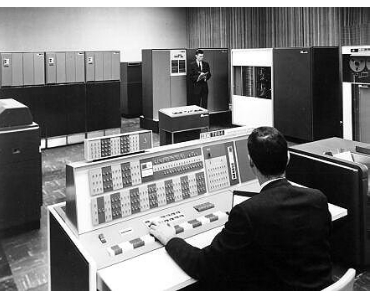
\includegraphics[width=.8\linewidth]{IBM7094.jpg}
  \end{sidecaption}
\end{figure}

D'un point de vue technique \textcite{Haggett1969} cite comme véritable point de départ dans la discipline la  démocratisation de l'accès à la ressource informatique après 1961, avec la diffusion d'une deuxième générations d'ordinateurs dans les grands centres de calculs, en partant notamment de la série IBM 7094, le CDC 3400 de Northwestern \autocite[3]{Marble1967}, des ordinateurs que l'on imagine beaucoup plus accessible et performants que la précédente série IBM 604 et 650 qui suivront (voir \href{http://www.aag.org/cs/garrison}{@Garrison}...

En réalité, malgré l'apparition début des années 1970 des premier postes informatique individuels, l'expression de la simulation de modèle à la fin des années 1960 est toujours limité par des problématiques humaines, techniques très fortes \autocite{Haggett1969} \autocite[387]{Marble1972}, dont on peut constater dans les ouvrages inter-disciplinaires vu dans la section précédente, qu'elle ne touche en réalité pas que la géographie \autocite{Guetzkow1972}.

Dans une période ou les compétences informatiques nécessaires à la programmation se font encore très rare, les langages de programmation multiples et peu stable, le matériel coûteux et peu disponible, des packages de programmes disponible dans les universités sont quand même peu à peu publiés. Des pionniers comme Marble ou Tobler mettent à disposition courant des années 1960 différente routines informatique en libre accès \autocite{Haggett1969}  (\textcite[3]{Marble1967} parle de 150 routines développés jusqu'à 1967, cela seulement à Northwestern dans le département géographie), le premier package pour les science sociales SPSS (\foreignquote{english}{Statistical package for Social Science}) date quand à lui de 1968 \autocite{Barnes2011} , date à laquelle sort également l'ouvrage \foreignquote{english}{best-off} de Berry et Marble \foreignquote{english}{Spatial Analysis: a Reader in Statistical Geography}, qui offre les derniers programmes et donne ainsi corps à la statistique spatiale. 

Autant d'éléments de contexte historique qui donne un aperçus rapide des difficultés et surtout des efforts déployés par les pionniers Marble, Pits et Bowlby pour opérationnaliser les premiers travaux d'Hagerstrand \autocite{Hagerstrand1953, Hagerstrand1967a} et par la suite ceux de Morrill. 

Finalement les universitaires géographes, plus spectateurs qu'acteurs sur le développement des \textit{large scale models} \autocite[8]{Batty1976} \autocite[11]{Batty1994}, semblent attendre beaucoup des retombées de ces grands programmes \autocite{Haggett1969} qui dispose de moyens humains et économiques importants pour développer des programmes et collecter des données.

Si le requiem de \textcite{Lee1973} a bien eu un effet non négligeable sur la construction et la publication de tel modèles du coté des planifieurs \footnote{Seulement trois modèles seront publiés dans le même journal à la suite de cet article ...}, force est de constater que la construction de simulation pour la théorie urbaine ne disparaît pas dans cette période \autocite[11-12]{Batty1994}, et s'appuie au contraire sur l'apprentissage de ses échecs pour se réinventer dans les années qui suivent. A ce titre, \textcite{Harris1994} soulève dans une relecture très critique de l'article de Lee, l'obfuscation ou la méconnaissance de l'auteur vis à vis des débats qui agite déjà depuis plusieurs années la simulation de modèle urbains \autocite{Wilson1970, Orcutt1957, Harris1968}. Ce faisant, Harris accuse Lee d'enfoncer des portes ouvertes et de porter des accusation que certains jugeront par la suite prématurés vis à vis du préjudice subit, touchant à coeur une discipline encore bien jeune et en phase d'apprentissage, d'à peine une décennie. \autocite[p11]{Batty1994}.

Ce mouvement de modélisation doit faire face à l'expression de ces limitations pour se reconstruire, limitations dont on sait par avance qu'elles ne seront pas seulement levés par la seule amélioration des techniques. Ainsi pour \autocite[11]{Batty1976}, plus importants que tout les autres problèmes, c'est la révélation dans l'observation de cette richesse et de cette complexité d'interactions des facteurs causaux à l’œuvre dans l'évolution et la structuration des phénomènes urbains qui va le plus impacter sur la réévaluation des formes de modélisation dans ce domaine.

Une des réponses à ce renouveau vient du le milieu universitaire. Bien que peu sollicité \autocite[9]{Batty1994} pour la construction de ces modèles qui sont avant tout conçu dans le cadre d'une stratégie efficace de plannification, et ou l'efficacité l'emporte le plus souvent sur la curiosité scientifique, celui n'est pas en reste de ses propres travaux. Ainsi différentes équipes de développements sont déjà bien identifiées dans la communauté universitaire des économistes comme \textcite{Orcutt1960} et son premier modèle micro \foreignquote{english}{bottom-up} développé aux Urban Institute, les démographes sur les modèles de migrations inspirés des travaux d'Orcutt comme REPSIM, puis POPSIM; et enfin l'apport de \textcite{Forrester1961} sur l'optimisation industrielle, une des branche opérationnelle d'inspiration la plus directe du projet systémique au début des années 1960 \autocite{Cohen1961} \autocite[911]{Shubik1960b}.

% et Hagerstrand ? 
La \enquote{micro simulation} initié par Orcutt, qui semble effectivement passer outre l'extinction annoncé par Lee en 1973, rencontre même un certain succès durant toute les années 1970 comme en témoigne la mise en place de nombreux programme nationaux au début des années 1980. \autocite{Baroni2007} Une réponse à cette survie peut être avancé dans le positionnement innovant d'Orcutt pour face aux résultats décevant des \textit{Large Scale Models} de son époque, opérant pour la plupart à un niveau macro et fournissant des résultats hautement aggrégés difficile à exploiter dans un cadre prédictif, et finalement peu représentatif de la diversité des systèmes économiques \autocite{Birkin2012} \autocite{Baroni2007}. Si les critiques de Lee peuvent pour la plupart être mobilisé pour critiquer les modèle issue de la micro-simulation (complexités des modèles, absence d'objectifs clairement posés, volume des données à mobiliser, complexité des calculs, coût de construction, absence de résultats, etc.), il n'en reste pas moins que la proposition d'Orcutt introduit avec une approche plus \textit{bottom-up} une dimension explicative absente jusque là. En répondant à l'observation de Lee sur l'absence d'extraction de connaissance micro quelque soit la complexité injecté dans les modèles macro, Orcutt ouvre d'une certaine façon la voie à des développements théoriques beaucoup plus riche que ne le permettait à l'époque les seuls modèles Macro, faisant ainsi de son modèle un instrument pour \foreignquote{english}{consolidating past, present, and future research efforts of many individuals in varied areas of economics and sociology into one effective and meaningful model; an instrument for combining survey and theoretical results obtained on the micro-level into an all-embracing system useful for prediction, control, experimentation, and analysis on the aggregate level} \autocite[122]{Cohen1961}.

De plus cette crise qui on l'a vu touche avant tout les institut de planification couvert par la RAND va fournir \textit{post mortem} le terreau enrichissant nécessaire à la transformation d'une discipline dont le rayonnement dans la communauté scientifique à l'international ne va aller qu'en s'amplifiant après 1970 (voir la carte des foyers ou sont pratiqués la modélisation urbaines en 1980-90 dans \autocite{Wegener1994}).

Autre pistes de développement pour ces universitaires, les retombées de certains modèles produit par en partenariat avec la RAND ayant fourni de bon résultats, comme celui de Lowry \autocite {Lowry1964}, vont fournir la base de nouveaux travaux mettant en perspective l'influence ou les progrès d'autres courants disciplinaires en contact avec la géographie. 

Ainsi la \foreignquote{english}{social physics} de \autocite{Wilson1970} est considéré comme un moment important dans le renouveau des modèles urbains \autocite{Griffith2010}, de la même façon que le projet systémique des cybernéticiens d'abord et de Bertalanffy ensuite, qui contient dans son expression tout les outils conceptuels et opérationnels permettant la modélisation et l'étude d'un objet au travers de ses interactions complexes, comme la ville \autocite{Forrester1969} \autocite[11]{Batty1976, Batty2001} mais aussi plus généralement tout autre objet géographique \autocite[27-28]{Pumain2003} \footnote{ Pumain liste au moins trois intérêts qui découle de cette phase d'acquisition du projet systémique : a) le dépassement de l'opposition idiographique et nomothétique, b) l'histoire et les particularités des entités géographiques vues comme expression originale de trajectoires et de bifurcations, c) le dépassement de la rigidité des trajectoires biographiques historiques par l'emploi des simulations}

Mais il serait réducteur de parler de ce renouveau qui touche une catégorie de modèle bien spécifique, les modèles urbains, sans évoquer également les travaux précurseurs d'une autre branche de développement universitaire, qui semble intégrer là aussi tout à la fois les influences du courant néo-positivistes que les influences systémiques. %% FIXME %%

Si les années 1970 souffre moins de cette problématique technique, du fait en partie de la simplification des modèles, les problèmes relatifs à la validation des modèles restent eux tout à fait d'actualités. Un témoignage recueilli dans un échange de mail en 2013 avec Marble, interrogé au sujet de la suite des problématiques de validation des modèles de simulation détaillés dans son article de 1972 \autocite{Marble1972}, conforte ce point de vue : \foreignquote{english}{As I recall, the situation in the 1980's had not changed very much. Simulation in human geography did not last long. Much of this was the result of a lack of computer capacity. Simply replicating Hagerstrand's diffusion model proved difficult and our attempt to inject a more explicit temporal element just would not work due to the computational load.}

Un témoignage à mettre en relation avec les tentatives des géographes Français des années 1980, ou les problématiques de validation sur des modèles, opérant pourtant sur des populations agrégés, restent largement limités par des problématiques de calculs, la nécessité d'intermédiaire humain et technique. Les analyses statistiques doivent être adapté à la dimension spatiale, % A détailler un peu %

%%FIXME : A MODIFIER POUR COLLER AVEC LE PARAGRAPHE PRÉCÉDENT %%

L'existence de ces deux courants parallèle dont on mesure mal l'inter-dépendance est relaté par de multiples auteurs. Mais c'est chez \autocite{Wilson1972} que l'on retrouve peut être le mieux exprimé cette dualité entre les deux courants, avec d'une coté une géographie théorique issue de la branche \foreignquote{english}{Models in Geography} qui manque de données, s'avère limité dans son expression opérationnelle, et porte selon lui encore trop l'emphase sur l'induction statistique et pas assez sur la démarche hypothético-déductive pour former des modèle \footnote{Modèle est ici synonyme pour lui de théorie} ; et à l'inverse opposé la branche instigatrice des \textit{large scale models} qui fait (trop) usage des dernières techniques, dispose de large données, mais s'avère incapable du moindre résultats car trop peu regardant sur l'usage des théories \autocite[10]{Batty1994}. On peut ne pas être d'accord avec ce que dit Wilson par ailleur dans cette article, mais il fait ici figure de précurseur dans sa volonté de lié les deux approches, tant il semble bien conscient que la réussite de la démarche de construction des connaissances en géographie tient avant tout de la complémentarité entre cette approche inductive et l'approche hypothético-déductive pour vérification.

Nombres de problèmes vont par la suite se débloquer dans le courant des années 1970 en géographie.

% Ajouter reférence denise complexité, qui permet de faire le pivot dans l'argumentation, sur systémiquer qui permet de dépasser idiographique vs nomothétique (à vérifier dans le texte)

Le mouvement du professeur Orcutt \autocite{Orcutt1957}, mais aussi celui de Forrester \autocite{Forrester1961, Forrester1969} vont par la suite amener chacun à leur manière une nouvelle dimension explicative et l'ajout d'une dimension temporelle dynamique plus à même d'aborder cette complexité qui fait défaut aux théories actuelles. \autocite[p295]{Batty1976}

Ainsi les progrès fulgurants de l'informatique, l'apparition de nouveaux langages exclusivement orienté pour la simulation comme Dynamo, la prise de conscience tout au long des années 1960-70 des défaut de cette première génération de modèles, et les changement d'objectifs de la discipline \autocite[12]{Batty1994} \autocite{Boyce1988} autorisent (voire recommandent) la formation de nouveaux modèle. Ceux ci sont concus comme plus parcimonieux, autorisant les démonstrations plus abstraites \autocite{Forrester1969}, plus orienté vers la compréhension des mécanismes à l’œuvre que sur la prédiction (un retour sur les modèles théoriques est opérés), intégrant plus facilement l'hétérogénéité dans la nature des dynamique (rétro-action, non linéarité) des processus \autocite{Forrester1969} \autocite{Wilson1970} \autocite{Allen1975}, et ouvert à l'intégration d'autres dimensions explicatives à l'oeuvre dans la formation des processus, comme ceux déjà exploré l'individu et le temps \autocite{Hagerstrand1967a} \autocite{Orcutt1957} \autocite{Forrester1961}. En lisant les articles de Pred, d'Olsson \autocite{Olsson1969} \autocite{Olsson1970}, de Curry, on percoit chez les nouveaux économistes spatiaux cette volonté de changement, avec la reintroduction de la stochasticité et des modèles probabilistes, l'intégration du temps dans les modèles, mais aussi les causalités multiples.

% PLUSIEURS points développement méthodologiques accompagnant renouvellement théoriques accompagnant nouvelle géographie : Hagerstrand , Orcutt -> causalité + individualisme méthodologique,  Forrester -> complexité
% Hagerstrand premiere utilisation montecarlo en science sociale, vient a Washington et rencontre Morril... qui pour Benko Stromayer marque troisieme theme dominant le bouleversement quantitatif) Gould2004

% simulation permet de développer cette causalité ...
% Systeme dynamique, non linéarité, permet avancée fondamentale dans les questionnements, révélateur aussi de l'apport des techniques / méthodologies...
% Basculement vers explicatif !

\subsection{Les techniques évoluent mais les problématiques fondamentales persistent}

Heureusement, les capacités de calcul informatique et les méthodes de modélisation multi-échelles des informations spatio-temporelles se sont bien développées, en parallèle et en réponse à ces nouveaux défis. Parmi les sciences humaines et sociales, les géographes sont aujourd'hui particulièrement présents dans l’expérimentation et la mise au point méthodologique, qu’il s’agisse des les appliquer à des données environnementales (Kanevski, Delahaye, Douvinet) ou à des problèmes de géographie urbaine (Batty, Banos, …Ruas) ou régionale (Wilson, Dauphiné, White, Engelen, Daudé) ou encore à l’analyse de réseaux (Rozenblat). 

Les systèmes complexes sont bien entendu aujourd'hui au cœur des interrogations en sciences humaines et sociales, dans la mesure où il est connu depuis très longtemps dans ces disciplines que les interactions en jeu ne sont pas linéaires \todo{ (Morin, 200 ) }  (Morin, 200 ), que des individus engagés dans des processus collectifs sont susceptibles de donner lieu à des phénomènes originaux à l’échelon macroscopique (Schelling, 1978) \todo{ (Schelling, 1978) }, et que les situations initiales ou les effets de contexte sont parfois aussi déterminants que les modalités qui règlent les échanges entre les individus, suscitant des évolutions où la \foreignquote{english}{path dependence} \todo{ (Arthur, 1994) } (Arthur, 1994) ou \enquote{enchaînement historique} joue un rôle très important, en limitant les expressions des dynamiques possibles.

Suivant une remarque emprunté à Gould \autocite[31]{Gould2004} \enquote{[...] il faut bien se rendre compte que la formulation de questions et les avancées méthodologiques sont les deux faces d'une meme piece}. Banos \autocite{Banos2013} compte jusqu'à quatre étapes majeures ou progression technologique rime avec évolution et remise en question des questionnements théoriques. Ainsi, tout comme la systémique et la formalisation mathématique avait permis la découverte des trajectoire complexes mais cohérentes des objets géographiques, soumises non plus à des rencontres locales mais à des contingence génératrice de bifurcations dans la dynamique des villes \autocite[137]{Pumain2002}, l'apport de la modélisation multi-agent des années 1990 pousse elle encore un peu plus loin la transformation. \autocite{Sanders2007}

%Avec l'apparition des modèles agents comm en géographies les nouvelle approches ouvrent de nouvelles voies à la pensée et au questionnement littéralement impensables auparavent, on peut citer par exemple la programmation déjà linéaire, qui souleve (cf Leslie Curry, aussi cité ailleur par Hagget je crois) + introduction de Gould1970 "The intellectual revolution in geography since the middle and late fifties rests upon two main supporting pillars" 

Les modèles d’agents employés en géographie ont la particularité d’avoir été développés non seulement pour des simulations d’agents individuels, par exemple pour simuler la diffusion d’épidémies dans un territoire urbain ou régional ou sur un réseau (Banos SRAS, Badariotti, Laperrière, Eubank…) ou la diffusion d’innovations (Daudé), la propagation d’incendies (Langlois), ou encore pour éclairer les choix résidentiels (Bonnefoy…) mais ont démontré l’intérêt de modélisations fondées sur des entités plus vastes (villes, régions, voire états du monde) pour examiner les possibilités d’émergence à partir de leurs interactions à des niveaux géographiques plus larges. 

%Le laboratoire Géographie-cités a été pionnier dans l’application à la géographie des systèmes multi-agents, notamment avec la série des modèles Simpop réalisés en collaboration avec des informaticiens (Bura et al., 1996, Sanders et al., 2007, Pumain, 2012) mais aussi avec des modèles d’agents développés directement avec des logiciels simplifiés comme Netlogo (Banos…). L’évolution des modèles ne se limite pas à l’emploi de logiciels mais participe plus généralement des réflexions de la communauté scientifique intéressée par les systèmes complexes. Le GDRE S4 (Simulation Spatiale pour les Sciences Sociales) a par exemple inscrit son action parmi les premiers projets de l’Institut des Systèmes Complexes de Paris-Ile-de-France (ISC-PIF) fondé par Paul Bourgine \todo{ (ref) }. L’UMR  Géographie-cités est devenue en 2011 l’antenne  de l’Institut des systèmes complexes à l’Université Paris I et acquiert du matériel pour sa propre autonomie de fonctionnement.

Toutefois, là ou on aurait pu attendre une amélioration sur les questions de la validation des modèles de simulation agents, on se rend compte qu'un certain nombre de problématiques persistent et limitent toujours la diffusion des modèles en dehors du cercle bienveillant de l'inter-disciplinarité \autocite{Richiardi2006}. Ce problème, loin d'être un isolat touchant uniquement les sciences humaines et sociales, existe dans d'autres disciplines, comme c'est le cas en écologie, où même lorsque les modèles sont publiés, l'absence de protocole pour répliquer, evaluer le modèle est courant \autocite{Grimm1999}.

A juste titre donc, l'absence de protocole pour l'évaluation des modèles est cité comme un des nombreux écueils avec lequel se bat toujours la discipline \autocite{Heath2009}, comme en témoigne les discussions réccurentes de nombreux auteurs sur un sujet dont la complexité touche à une dimension technique, que méthodologique ou philosophique. Autant d'auteurs \autocite{Richiardi2006} \autocite{Fagiolo2007} \autocite{Moss2008} \autocite{Windrum2007} \autocite{Barlas1996} \autocite{Amblard2003} \autocite{OSullivan2004} \autocite{Doran2000} \autocite{Crooks2012} \autocite{Rouchier2013} dont il faudra développer les discussions.  

Un problème qui met un peu plus en danger des communautés de chercheurs dont on sais déjà leur isolement : archéologie, sociologie \autocite{Manzo2007}, et économie \autocite{Lehtinen2007} \autocite{Richiardi2006} pour n'en citer que quelqu'une. 

cette critique récurrente de l'outil sur le plan de la scientificité, une faiblesse qui constitue toujours un danger pour la pérénité des pratiques inter-disciplinaire autour de la simulation agents \autocite[220]{Squazzoni2010}, a tel point que la communauté se dote de guides de survie pour se protéger des sceptiques. \autocite{Waldherr2013} Est ce là le seul fait d'une mauvaise communication autour de notre discipline comme le laisserait penser la lecture de ces travaux ? 

De plus ce manque de crédibilité, qui prend souvent la forme de serpent de mer \footnote{ On pensera nottament à cette fameuse question, récurrente lors des assemblées : \enquote{Avez vous validé votre modèle?} et si oui, \enquote{Quelle connaissances pouvez vous en tirer vis à vis de votre discipline ?} \autocite{Amblard2006} } opère dans un cercle vicieux où l'absence d'évaluation nourrit une perpétuel remise en question de cet outil et de sa scientificité. %% REPETITION



Cette étape de validation, l'écueil le plus important surement, est pourtant souvent évoqué comme une étape cruciale dans bon nombres de guides méthodologiques pour \enquote{la bonne construction des modèles}, qu'il soit ancien \autocite[195]{Beshers1965} \autocite{Naylor1966} \autocite{Naylor1967}, récent \autocite{Amblard2006} \autocite{Gilbert2008}, technique ou atechnique. 

Malheureusement, cette étape est très rarement \footnote{On soulignera à ce titre la qualité de l'ouvrage de Railsback et Grimm \autocite{Railsback2012}, les deux auteurs prenant le temps de développer ces aspects en détail avec des exemples} mis en oeuvre dans des exemples concrets \footnote{On pourra se référer à la critique cinglante de \autocite{Manzo2007a} vis à vis du guide méthologique établit récemment par \autocite{Gilbert2008}, particulièrement muet sur la question de la validation du modèle qu'il défend dans l'ouvrage... Si même les auteurs aussi cités et reconnus que Gilbert, qui ont la chance de publier pour la première fois cette méthode dans une collection aussi reconnu (\textit{Sage Quantitative Applications in the Social Sciences}), ne donne pas l'exemple, que doit on attendre des plus jeunes recrues s'essayant à cette technique ?}, et cela en partie du fait de la nature tout à fait contextuelle de cette étape, cf.\enquote{Amblard2006}{"[...] les questions pour  la validation des modèles ne devraient jamais être abordées en dehors des questions relatives à leurs usages"}

Il ne serait alors pas outrancier de de tenter ici une comparaison entre la désillusion vécu courant des années 1970, et la situation tel qu'elle apparait en 2014. Car sur ce point, un regard sur l'histoire passée de la simulation dans les sciences sociales n'est pas fait pour nous rassurer, la plupart des problèmes cités comme facteurs limitants dès les années 1970 recoupent encore aujourd'hui tout ou partie de nos problèmes actuels. On pourra arguer que certaines problématiques, comme les problématiques techniques d'accès aux ordinateurs, ou aux programmes ont quasiments disparu. Certes oui, mais de nouvelles problématiques, de même nature, sont apparus, et s'avère tout autant limitantes dans le but poursuivi. La problématique de l'accès et de l'utilisation d'une puissance de calcul nécessaire et suffisantes pour l'exploration des modèles n'est ainsi qu'une translation à un niveau supérieurs de problématiques plus anciennes...

%En forte interaction, ceux ci peuvent être rapportés à au moins trois dimensions explicatives, une dimension technique, une dimension méthodologique et une dimension institutionnelle, ce qui peut être explique pourquoi ceux ci n'ont jamais pu être totalement résolus dans le cadre d'une seule politique, d'une seule projet, ou d'une seule publication : faible nombre de modèles publiés et reproductibles, absence de publication décrivant des protocoles d'évaluation de modèles et des mises en application de ces protocoles, difficulté d'accès à l'information et à la ressource technique nécessaire pour l'exploration des modèles, stratégie de publication misant sur la publication de modèles déjà finalisés mais jamais appliqués de nouveau, manque de formations adaptées ou dédiées, confrontation avec des courants disciplinaires \textit{mainstream} ignorant l'activité modélisante, etc.

%La plupart du temps, ces papiers méthodologique pointent des arguments faisant état des limitations techniques, mais il apparaît de façon assez nette que la problématique de la validation des simulations et la lutte régulière pour reconnaître le caractère « scientifique » de la simulation et son intérêt pour dégager de la connaissance semble être un argument transerval dans les différentes disciplines et dans le temps.

%En reprenant notre argumentaire pour y exposer non plus le modèle non plus dans sa dimension uniquement technique, mais dans sa dimension de construit, de nouveaux objet d'étude apparaissent.
Ce qui semble être décrit comme une immaturité dans la méthode Agents \autocite{Heath2009} se rapporte en réalité à des pratiques qui dépasse largement l'utilisation spécifique de cette technique spécifique. La simulation agents en apportant cette nouvelle et importante flexibilité dans l'expression des problématiques de recherche, a pu certainement provoquer un effet de mode menant à des dérives, un état de fait qui ne nous fera pas oublier l'enracinement d'une bonne partie des critiques qui lui sont adressés, à tort ou à raison.

Compte tenu de cette persistance des problématiques dans le temps, au delà de l'évolution des techniques, il est fait ici un choix radical. En objectivant cette \enquote{démarche scientifique de construction de modèle} pour en faire un objet d'étude à part entière, et en laissant dans un premier temps de coté les supports techniques (modèles équationels, modèles agents, etc.), il est proposé dans cette étude de se concentrer sur la problématique de validation/vérification des modèles, une étape déterminante au coeur de la construction du modèle. 

Un retour sur la démarche de construction des modèles en géographie s'avère nécessaire pour comprendre les éléments qui nous ont échappés dans la continuité de cette problématique qu'est la validation des modèles. En s'appuyant sur les témoignage de \autocite{Batty2001, Pumain2003} on parvient très bien à décrire ce basculement opéré à la charnière des années 1960-1970, alors même que les géographes accède peu à peu aux concepts opérant dans le paradigme systémique \autocite{Harvey1969}, et que l'insuffisance de la démarche de découverte scientifique proposé par les néo-positiviste est pointé du doigt de façon générale \autocite{Simon1973} . 

En géographie, c'est d'abord l'échec du programme néo-positiviste comme programme opérationnel qui est flagrant. Celui ci est visible en au moins trois points : Le premier concerne le retournement opéré par Harvey \autocite{Harvey1969}, dont le livre phare \textit{Explanation in Geography}, censé faire une synthèse de la démarche explicative en géographie, avait été vivement critiqué \autocite{Gale1972} dans le très récent et sérieux journal \textit{Geographical Analysis}. Après une rédaction difficile et peut être même prémonitoire \autocite[47]{Barnes2006}, celui ci renie dès 1972 \autocite{Harvey1972} toute une partie de ses travaux et rejoint la fronde d'une géographie radicale émergente, elle aussi tout à fait critique envers cette démarche et le peu de preuve d'utilité de ces modèles théoriques hérités de l'économie \footnote{A ce titre, le projet d'Hagerstrand s'en tire beaucoup mieux, d'une part car l'auteur croit à une science profondément humaniste et transdiscplinaire \autocite{Bailly2000}, et d'autre part car il porte en lui ce projet de réconciliation entre l'individu singulier étudié dans sa trajectoire temporelle d'une part, et une vision plus générale résultats de l’agrégation de ces comportements individuels à un niveau sociétale d'autre part}.

Autre manifestation de cet échec, plus retentissante encore, est sûrement l'écho \autocite{Lee1973} des résultats médiocre d'une décennie de modélisation piloté par les instituts de plannification, fort coûteuse, appliqués aux systèmes urbains. Entre 1958-1968 aux États-Unis, un grand nombres de modèles théorique \autocite[7-9]{Batty1979} dérivés des modèles de l'économie spatiale naissante sont utilisés \textit{a priori} sur de larges corpus de données, et cela à des fins de prédictions plus que d'explication. Il faudra attendre plusieurs années par la suite pour que renaissent sous cette appellation des \textit{large-scale models} un tout autre programme de modélisation \autocite{Boyce1988}. Un parallèle peut donc être tenté entre d'une coté une démarche scientifique reconnue idéalisé \autocite{Besse2000}, alors dominante, dérivé de l'école néo-positiviste, à savoir le modèle Nomologico-Deductif et Hypothético-Deductif de Hempel-Popper, et d'un autre coté l'application décevante de modèle la plupart du temps statique, descriptif, à l'équilibre, et utilisés à des fins essentiellement prédictive sur de large collecte de données. 

Quel exemple plus marquant peut on trouver pour démontrer que la prédiction de systèmes aussi complexe que les systèmes urbains et par extension sociaux n'est pas compatible avec une démarche de construction des connaissances qui met sur pied d'égalité prédiction et explication ? (le fameux \enquote{Expliquer c'est prédire} de Popper). On s’intéresse plus à la description (le Comment ?) qu'au mode de production des phénomènes (le Pourquoi ?), les seuls pourtant à pouvoir donner une certaine intelligibilité aux lois que l'on utilise. \autocite[14-15]{Besse2000} Cet échec amène une partie des planificateurs à réviser des théories trop simplistes et surtout induit indirectement la nécessité d'un retour à une démarche inductiviste plus exploratoire \footnote{On notera par exemple le témoignage de \autocite{Boyce1988} lorsqu'il dit à propos des chercheurs engagés dans cette voie \foreignquote{english}{Some, including myself, turned to more empirically oriented research activities, perhaps in the hope of strengthening the foundation of future models}}, jusque là oublié.

Cette vision dogmatique d'une science réductionniste ou la \enquote{loi} seule pilote l’expérimentation n'aura pas tenu longtemps, et l’échec du néo-positivisme ne tarde pas à être annoncé dans le courants des années 1970. Le paradoxe entre cette science géographique qui cherche de plus en plus à étudier les interactions entre l'humain et son environnement, mais dispose seulement jusqu'à alors d'un modèle de causalité linéaire issue des sciences physiques, largement idéalisé, est finalement mis en défaut et abandonné par ses propre detracteurs \footnote {Hempel abandonne le modèle vérificanioniste en 1950-51, et le falsificationisme en 1965}.

Autre échec notable est l'échec de cette internationalisation de cette épistémologie, du moins en France, courant des années 1970. Claval ne note pas de réelle diffusion de cette épistémologie, qui provoque au regard de l'épistémologie post-vidalienne existante un certain rejet.. (retrouver la ref). Le débat épistémologique intéresse certes, mais selon lui les géographes francais sont alors bien trop occupé alors à intégrer les fascinantes et toutes dernières techniques quantitatives pour qu'une synthèse voit le jour sur le sujet.\autocite[27-29]{Claval2003}

Si Bertalanffy fut marqué par le néo-positivisme à une période de son étude \footnote{Fait étonnant Victor Kraft est un géographe, philosophe proche du cercle Viennois, mais tenant d'un point de vue original rapport à ce courant. Celui forme des géographes très tôt en allemagne à des méthodologies quantitative (1929). En 1926, Bertalanffy proche du milieu viennois à ce moment, emprunte à celui ci en 1926 la méthode hypothético-déductive \autocite[342]{Pouvreau2013}. Une boucle intéressante semble alors se former entre i) Kraft dont la formation est inspiré par Pleck, un professeur allemand inspiré de la méthode déductive de Davis, ii) Kraft indirectement amené à participer au débat Schaefer-Hartshorne du fait de son travail ainsi cité, et iii) le fait que Bertalanffy va ensuite nourrir les travaux de Chorley qui prend la suite des études de Davis en géomorphologie...}, celui ci subit par la suite de très violente critiques de la part de plusieurs membres, en Allemagne, puis aux états-unis, marquant un profond désaccord qui ira en grandissant par la suite \autocite[26-27]{Pouvreau2006}.

Les apports du paradigme systémique offre tout les concepts nécessaires pour sinon résoudre, au moins admettre un premier dessin de cette complexité \autocite{Dauphine2003}, avec à la clef un effet libérateur en géographie pour bien des raisons évoqués par \textcite[27-28]{Pumain2003}, qui tiennent aussi bien compte des apports techniques que méthodologiques de cette discipline, deux objet dont la trajectoire est intimement lié. 

Cette diffusion de la systémique dans la géographie semblent se faire par deux voies, d'une part celle des isomorphismes, et d'autre part celle d'un nouveau concept de pensée de la complexité.

Encore peu connu des géographes à la fin des années 60 si on en croit Harvey \autocite{Harvey1969}, la géographie dispose déjà pourtant de \enquote{passeurs de connaissances} solides à cet époque, dont la filiation est souvent à chercher dans les mouvements systémiques (Cybernétique ou GST). Sans compter que la géographie n'est pas complétement ignorante des relations qu'elle entretient avec les mathématiques, ne serait ce que pour la cartographie ! Ces transferts de concept, heureux ou malheureux, d'une discipline à l'autre se concrétise dans une une révolution qui doit non pas tant inventer des loi ex nihilo, mais plutôt extraire ou reconstruire depuis ces fondements historiques la part de géographie propre à ces isomorphismes afin d'établir plus explicitement ces \enquote{loi} qui lui manquent tant. 

On citera entre autres sur l'adaptation du modèle gravitationnel au modèle de population, sur les travaux initiaux des géographes Ravenstein (1885) et Levasseur (1889), puis l'économiste Reilly (1929), se greffent les travaux de Warntz (géographe) et Stewart (physiciens) \footnote{Déjà connu des géographes par sa publication de 1947 qui pose l'isomorphisme entre population et gravité, Stewart fait probablement naitre une certaine curiosité chez certain pionniers. Ullman s'avère par exemple être un fin lecteur \autocite[61]{Glick1988} et \href{http://nwda.orbiscascade.org/ark:/80444/xv01385}{@Correspondant} de Stewart. Warntz de son coté est un géographe plongé dans l'inter-disciplinarité. Financé par l'ONR il est présent à l'AGS (American Social Geography), au département de science régionale de Pennsylvania's, et dans le département d'astro-physique de Princeton où il est amené à collaborer régulièrement avec Stewart, avec qui il \href{http://rmc.library.cornell.edu/EAD/htmldocs/RMM04392.html}{@Correspond} aussi après guerre. \autocite{Barnes2006}.

C'est Wilson, un autre physicien, qui viendra en 1970 améliorer le modèle en y introduisant la notion d'entropie, une notion qui doit sa filiation ici à l'analogie entre théorie de l'information et thermodynamique réalisé par les cybernéticiens.

On connaît également les relations étroites entre les travaux pionniers de Lotka et les géographes et statisticiens de toute nationalités, comme Hägerstrand qui semble avoir été explicitement inspiré par sa vision de la démographie \autocite[95]{Claval2007} pour définir l'ancrage spatial de ses individus; une admiration que l'on retrouve également dès 1930 en France chez les statisticiens démographes, mais aussi dans la littérature américaine qui apparait déjà largement inter-disciplinaire \autocite{} . Hors c'est bien Alfred J. Lotka, un mathématicien, chimiste et statisticien qui reprend et théorise le premier le point de vue de Boltzmann qui va largement influencé par la suite Bertalanffy dans la formation de sa \enquote{systèmologie générale} \autocite[178]{Pouvreau2013}, notamment par ces études de la démographie des populations et des flux de matières dans le monde biologiques \autocite[545-546]{Pouvreau2013}

On retrouve également avec la loi de Zipf-Auerbach une filiation indirecte avec la physique de la thermodynamique du début du XX ème siècle. C'est en effet le physicaliste Auerbach \footnote{ Si on en croit \autocite[87]{Pouvreau2013} Auerbac est convaincu que le progrès en biologie ne viendra que de l'explication entièrement physique des phénomènes biologiques} qui s’intéresse en premier à l'application sur des villes de l'effet d'inégalité soulevé par Pareto dans les population.\autocite[94]{Rosser} Il donne naissance à la loi Rank-Taille  qui montre que le produit de la population par le rang de la ville dans la hiérarchie est une constante. Une analyse repris et développé par Zipf dans une étude lexicologique, et qui lui permet en conséquence d’asseoir un peu plus son universalité, ce qui explique entre autre la confusion dans l’appellation. L'observation dans des espaces et des temporalités très différentes \autocite{Pumain1997} de cette distribution rang-taille comparable à une loi puissance ou une loi log-normale ouvre, à condition qu'on s'attache non pas à la finalité de l'objet lui même, un champs d'étude très vaste. On retrouve là une similarité avec l'étude systémique des organismes vivants, et on peut se demander si n'y a pas dans cette régularité sous forme de "finalité observable" une forme universalité qui pousse à formuler un rapprochement avec les moyens d'explicitation développé par Bertalanffy pour comprendre cette directivité des processus qui caractérise la formation de tout organismes biologiques. Une même type d'analogie sera développé avec la loi d'allométrie découverte en biologie, et reprise par la suite en science sociales.

L'équifinalité comme téléologie dynamique est permises du fait de l'interaction dynamique des éléments, et non pas de la structure initiale en place, sinon comment expliquer sa complexification progressive dès lors qu'on admet l'irréversibilité des processus associé au temps ? On comprend mieux dès lors l'attrait des géographes pour tenter d'expliquer, tout comme les biologistes le font, les mécanismes à l'origine de cette "régularité".

\autocite[114]{Pouvreau2013}
Tout processus d’équilibre peut être formulé téléologiquement [...] Toutes les lois systémiques ont
la particularité que ce qui apparaît pour l’ensemble du système comme un processus causal
d’équilibre peut être formulé téléologiquement pour les parties 1 .
Ce qui correspond à un processus causal d’équilibre apparaît pour la partie comme un événement
téléologique, en ce que l’action de cette dernière semble dirigée vers le « but » consistant à prendre
sa place « convenable » dans le tout 2


Enfin la crise des années 1970, et le retour à des modèles plus sobres, que l'on espère mieux maitrisé pour évoquer une complexité des objets géographiques.

dont on délaisse les aspects théorico-mathématiques globalisant et unificateurs trop complexe

et qui va continuer par la suite avec les travaux de Sanders sur Lotka Volterra,   dont on connait \textit{a posteriori} l'influence qu'ils auront par la suite à l'international et en France (Hagget, Chorley, Berry, etc.). Malgré tout, durant la décennie 1960-70, et malgré l'incompatibilité  évidente entre programme systémique et néo-positiviste, malgré la collaboration entre Bertalanffy et Chorley en 1962, personne ne semble avoir eu le temps de développer une telle critique dans cette période, ce qui est en quelque sorte révélateur de l'intensité de l'influence que peuvent avoir des penseurs comme Bunge ou Harvey dans la communauté anglaise. \autocite[123]{Unwin1992}...

D'un point de vue des concepts ..... .... ... blabla ... 

Pour Batty \autocite{Batty2001} \autocite[13]{Batty2008} c'est le modèle de Forrester \autocite{Forrester1969} qui polarise le mieux ce changement de perspective dans la démarche de construction des modèles. Provenant d'une toute autre source que les modèles urbain réalisé jusqu'à la fin des années 1970, celui ne va pas sans déclencher au mieux une certaine curiosité \autocite{Lee1973} , et au pire un véritable raz de marée de critique, d'abord chez les géographes\autocite{Tobler1970a} mais aussi de la part du grand public, entraînant parfois des réactions violente tant l'affaire est médiatisé \autocite[9]{Forrester1989}. 

D'un point de vue interne, le modèle \textit{Urban Dynamics} n'introduit pas tant d'originalité par rapport aux éléments acquis par la rencontre entre la vision d'Hagerstrand et les pionniers universitaires systémistes 10 ans auparavant, les premiers modèles de simulation qui implémente la dimension temporelle, stochastique, dans le premier langage Fortran (le seule langage scientifique de l'époque) étant daté d'avant 1965. Plus que sur les aspects géographiques, le modèle étant aspatial, \autocite{Batty2001} nous fait remarquer que c'est sur le point de la validation que la polarisation du débat s'effectue; car comment valider un modèle qui ne s'appuie sur aucune données autres que des valeurs de paramètres ?

A voir la modélisation comme un laboratoire virtuel parfait pour l'expérimentation, pourquoi ne pas pousser l'analogie jusqu'à rétablir l'équilibre entre théorie et expérimentation dans la construction des connaissances ? C'est un peu le choix établie par les tenants de l'abduction,  en réaction du modèle fermé sur les loi de HD - ND de Hempel-Popper propose le rétablissement d'un autre processus d'inférence souvent nommé par les anglo-saxon, IBE ou \foreignquote{english}{Inference to Best Explanation}. La surprise comme moteur de nouvelle découverte, surprise dont on se rend compte avec Morgan2005 qu'elle est au coeur d'un question épistémologique propre à la simulation.

impossible si on se place dans la stricte boucle fait . Pourquoi ne peut on pas prendre encore un peu plus de hauteur, et proposer un deuxième niveau de surprise, celui cette fois ci des outils, qui comme on a pu déjà le sous entendre dans le développement de ces introduction, joue un rôle tout aussi important dans le dévoilement de nouvelles questions. Pour reprendre la métaphore développé par Arnaud Banos \autocite[22]{Banos2013} à ce sujet, que se passe t-il si on remplace la machette utilisé pour l'exploration de l'aventurier dans cette jungle des hypothèses, son expérience ne risque elle pas d'être tout à fait différente ? Une lame qui devient tronçonneuse ne donne elle pas à voir un espace-temps tout à fait différent ? et un gps ne lui permettrait il pas de mieux savoir par quel endroit est on déjà passé ? Un équipement fait de géo-visualisation, de géo-computation, dont Arnaud Banos et d'autres avant lui ont développés pour y voir plus clair dans les choix que tout modélisateur est amené à prendre dans la construction d'un modèle.

Forrester donner à voir avec son langage graphique la structure causale de son modèle, une première qui démontre aussi la puissance d'un outils dans la démocratisation et la diffusion des techniques mais aussi des théories (systémique). L'analyse systémique aurait elle eu un tel succès si elle n'avait pas trouvé par l'usage de ces langages graphiques un nouveau crayon, qu'il faut encore apprendre à bien manier, pour organiser cette complexité ? Car Forrester ne fait pas que mettre en lumière avec un langage graphique adapté des éléments de vocabulaire de la cybernétique, il offre avec son langage DYNAMO le pendant opérationnel de celui ci, qui de graphique devient informatique. 

Peut on donner à présent le même langage graphique pour donner à voir la structure de nos expérimentations, une idée qui n'a rien de récente, et s'avère déjà largement utilisés pour visualiser toute sortes de chaîne de traitements, suivant des buts aussi varié qui vont de l'expérimentation artistique à l'expérimentation statistique.

Les géographes n'en reste pas là pour la plupart, et s'intéresse à la machinerie mathématique sur lequel s'appuie ce langage, qui reprend principalement les principes de l'école mathématiques des systèmes dynamiques, encore en pleine construction dans les années 1970, avec les apports des tenants physiciens de la systémique, entre autre l'école de Prigogine et l'école de Haiken.

%La démarche de construction de connaissance opéré dans l'activité de modélisation procède à une transformation dont \autocite{Forrester1969} est en quelque sorte le déclencheur, sinon le démonstrateur. En plein marasme \autocite{Lee1973} celui ci a le mérite de proposer une vision de la ville qui non seulement ne passe pas inapercu au yeux du public, mais qui rompt aussi avec la facon dont sont construit la plupart des modèles urbains existants. \autocite{Batty2001} En présentant un modèle complexe de simulation, aspatial, impossible à calibrer, \footnote{Ce modèle complexe sera largement critiqué à raison, mais aura quand même un impact important en engendrant une lignée de modèles \autocite[307]{Batty1976}.} qui s'appuie uniquement sur des données pour le paramétrage des hypothèses, et non pas sur une comparaison avec des données réelles, Forrester s'attire de très nombreuses critiques. Pourtant paradoxalement, c'est en montrant les effet contre intuitif de certaines politique publiques sur la ville que celui ci démontre l'importance et l'innovation de sa démarche. Il poursuit dans la même voie que d'autres avant lui \autocite{Orcutt1960} \autocite{Hagerstrand1967} et montre cette force de déduction que l'on peut tirer à partir de modèles dynamiques beaucoup plus parcimonieux que les équivalent statiques \autocite{Batty1976} et surtout il démontre avec la présentation d'effet contre intuitif le résultats de phénomène non linéaire jusque là difficile à imaginer avec les modèles statique à l'équilibre. 

Si le modèle déductif n'est pas à jeter complètement, il est au moins à relativiser \enquote{comme un des moyens possible} de la démarche scientifique en géographie, celle ci alternant le plus souvent entre phase exploratoire, et phase de déduction. \autocite{Sanders2000}

L'incapacité de ce modèle de démarche scientifique à assumer la complexité des systèmes urbains et sociaux nous amène tout droit à repenser l'évolution de cette démarche de construction dans ce qui fait au final la valeur d'un modèle aux yeux des scientifiques, ou du moins des géographes, à savoir sa capacité explicative.

Autrement dit, ce n'est pas tant \enquote{le modèle} que ce qu'il y a \enquote{dans le modèle} qui nous intéresse. \autocite{Sanders2000} 

=> Validation comme nouvel enjeu ?

\subsection{Comment construire des modèles de systèmes complexes qui participe à la production de connaissance}

En effet, la question de la \enquote{Vérification} des modèles, au sens philosophique du terme (valeur de vérité), reste indépassable du fait des multiples biais amenant l'observateur à toujours questionner la valeur de cette connaissance qui résulte d'un transfert entre les résultats d'un modèle volontairement imparfait (\enquote{simplifié}, donc réducteur par définition), et la \enquote{réalité} dans toute sa complexité \autocite{OSullivan2004}. Les termes \enquote{Vérification} et  \enquote{Validation} sont couramment rencontrés dans notre discipline, mais sous des acceptions différentes tenant souvent au transfert des terminologies entre ingénierie \autocite{Sargent1984} d\autocite{Balci1998} et philosophie, ce qui conduit à  des débats terminologiques sans fin \autocite{David2009}. 

Ainsi dans le cadre de notre étude, le terme \enquote{vérification}  \foreignquote{english}{[...] stands for absolute thruth } \autocite{David2009} \autocite{Oreskes1994} et se rapporte avant tout ici à la notion d'équifinalité \autocite{OSullivan2004} En dehors de toute considération technique, cette équifinalité qui décrit le fait que m-modèles créés par les scientifiques peuvent représenter la même réalité ( ou modèle de la réalité ), est tout à la fois un moteur et une limitation dans notre capacité de construction des connaissances. 

%ATTENTION, EXISTE AUSSI DANS LA PARTIE  1 EN C/C
L’existence de théories alternatives multiples est une constante dans l’histoire des sciences humaines. L'étude de l'objet social est un construit contextuel qui se nourrit d'une multiplicité des point de vues. C'est à ce titre que Jean-Claude Passeron \autocite{Passeron2006} nous met en garde contre une tentative de vérification des modèles qui serait décorrélée de tout contexte historique. Pour lui le faillibilisme poppérien qui se cache derrière la méthode hypothético déductive ne peut pas s'appliquer à la construction de théorie dans le cadre des sciences humaines et sociales. L'équifinalité est à ce titre un moteur permettant de confronter nos théories sur un objet social  qu'il est impossible de tout façon impossible de voir dans son unicité. 

Le processus de modélisation apporte une dimension supplémentaire à l'analyse de chacun de ces points de vue.Car il est hélas impossible de prouver par les modèles qu'il n'y a pas un tout autre ensemble de fait stylisés ou d'interactions qui soit capable d'arriver à la même observation, enlevant de fait toute unicité d’une explication \enquote{scientifique} au point de vue représenté par le modèle. L'équifinalité est donc à ce titre une limitation indépassable à la connaissance qui peut être déduite de nos modèles.

Le terme \enquote{validation} quant à lui est souvent entendu pour définir un état qualifiant la correspondance entre des observations empiriques et les sorties de la simulation. Compte tenu de la notion d'équifinalité, cet état de correspondance ne suffit pas à prouver que le modèle représente bien la \enquote{réalité}, dans la mesure où l’unicité de  cette adéquation peut être remise en cause par le jeu de nouvelles hypothèses. 

De façon plus générique la percolation du concept d'auto-organisation dans les sciences sociales et en géographie permet il me semble de donner une définition plus générale de ce type de sous détermination comme résultat de l'étude d'un processus à l'équilibre (On parle ici d'équilibre d'état, mais éloigné de l'équilibre thermodynamique, dans un système ouvert, cf. \textit{steady state} de Prigogine) sachant que tout \textquote[Pouvreau2013, 114]{[...] processus d’équilibre peut être formulé téléologiquement [autrement dit] Toutes les lois systémiques ont la particularité que ce qui apparaît pour l’ensemble du système comme un processus causal d’équilibre peut être formulé téléologiquement pour les parties. Ce qui correspond à un processus causal d’équilibre apparaît pour la partie comme un événement téléologique, en ce que l’action de cette dernière semble dirigée vers le \enquote{but} consistant à prendre sa place \enquote{convenable} dans le tout}. 

Peu importe donc l'étude de cette loi en tant que telle, puisque celle ci apparaît comme phénomène observable universel, ce qui intéresse le scientifique, ce sont les faisceaux d'hypothèses plausibles permettant d'approcher (ou pas, comme on l'oublie souvent, la négation est aussi explication !!) cette loi. La particularité de la géographie à ce niveau résidant avant tout dans sa capacité à maintenir ce faisceau d'hypothèse cohérent dans une diversités d'échelle et de temps, plus difficile à mobiliser dans d'autres disciplines.

Si on reprend l'objectif avancé par \autocite{Varenne2014}, \enquote{[...] la fécondité propre à la géographie de modélisation contemporaine et à ses différentes formes de manifestation tient en grande partie à sa capacité à affronter cette question de la sous-détermination, à comprendre qu’il ne s’agit plus tant pour elle de chercher des théories que de développer des modèles aux fonctions épistémiques multiples.} Si on comprend les enjeux d'un tel projet, se pose alors les moyens de sa réalisation; la systématisation des évaluations devient un outil au cœur de la construction des modèles, absolument nécessaire pour rendre cette fouille de modèles réaliste, et passé peut être à une échelle supérieure, celle de la construction et de l'étude de famille de modèles comme premier élément de réponse intégrateur de la pluralités des points de vues.

La notion de \enquote{laboratoire virtuel} traditionnellement limité à l'expérimentation du modèle mute, et se pare aujourd'hui d'une acception légèrement différente. Des chercheurs \autocite{Schmitt2014} \autocite{Amblard2003} ont voulu étendre cette notion pour y inclure également l'ensemble des méthodes et outils jugé nécessaire à l'étude de ce premier niveau d'expérimentation que représente la construction d'un modèle de simulation (la variation des hypothèses dans le modèle), désignant par ce fait un niveau supplémentaire d’expérimentation (la variation des outils et méthodes pour construire et étudier le modèle). 

%\begin{quotation} In fact, utility of simulation is sometimes confused with validity. The one refers to its usefulness for some purposes, whereas the other refers to its degree of correspondence with the real world. Since utility requires some degree of validity, some authors speak of a model as having been \enquote{validated} by some use to which it has been put. Validity of a model, however, is not and end in itself but merely a means of enhancing the utility of the model – and usually only up to a point. Both validity and utility are commonly matters of degree. […] While validity is the ultimate test of a theory, the ultimate test of a model is its utility.  \\ \sourceatright{ \autocite{Guetzkow1972}}\end{quotation}

%Comme \autocite{Amblard2006} le propose, nous remplacerons donc le terme de \enquote{Validation}, qui prête à confusion, par celui d’\enquote{évaluation}, qui n'est pas sans rappeler la notion d'utilité telle que définie dans la citation ci dessus.

\subsection{Une démarche pour systématiser l'évaluation des modèles}

Dans le cadre de cette thèse, nous défendrons une \enquote{évaluation} de modèle qui se confond presque complètement avec la méthodologie de construction qui la soutient. Cette \enquote{ validation interne } doit selon nous être systématisée au regard de la \enquote{ validation externe } qui mesure classiquement la correspondance entre données simulées et observées face à la question posée. C’est en cela que la démarche que nous proposons est \enquote{ systématique }. Les opérations nécessaires à la \enquote{ validation interne } telles que l'introduction, la modification, ou la suppression d'hypothèses, s’effectuent donc à la mesure de leur apport qualitatif et quantitatif dans l'explication de la dynamique globale sur laquelle se fonde la \enquote{ validation externe }. Autrement dit, c'est la recherche d'une cohérence qualitative autant que quantitative de la dynamique interne qui nous guide dans notre recherche de correspondance avec les données observées.

A ce titre, le recours au calibrage, et la recherche de cohérence interne dans les dynamiques pourraient passer pour une tentative de mieux définir par ce biais les processus en jeu dans un contexte réel. Pour \autocite{OSullivan2004} cet argument est encore un leurre, car toujours au vu de l'équifinalité, si ces procédures améliorent bien la connaissance du modèle, absolument aucune garantie ne peut être donnée sur la qualité et la transférabilité de cette connaissance pour l'étude de processus réel. Cela est d'autant plus vrai lorsqu'il s'agit de système complexes, dont la nature même empêche toute  mesure des dynamiques à l'oeuvre lors des processus d'émergence, et rend donc discutable toute comparaison possible avec des dynamiques simulées. 

\begin{quotation} It is clear that assessment of the accuracy of a model as a representation must rest on argument about how competing theories are represented in its workings, with calibration and fitting procedures acting as a check on reasoning. So, while we must surely question the adequacy of a model that is incapable of generating results resembling observational data, we can only make broad comparisons between competing models that each provide ‘reasonable’ fits to observations. Furthermore, critical argument and engagement with underlying theories about the processes represented in models is essential: no purely technical procedure can do better than this.  \\ \sourceatright{ \autocite{OSullivan2004}} \end{quotation}

% Un point de vue partagé par {Batty2001} ce qui permettrai d'introduire la notion de système complexe également !

Ainsi plus que les solutions techniques, c'est dans le processus de discussion et d'échange autour des hypothèses admises dans les modèles que notre connaissance sur les phénomènes réels est amenée à progresser. Par la mobilisation, l'hybridation, la confrontation de modèles ou briques de modèle issues d'angles de vues inter-disciplinaires,  on met en œuvre une grande discussion à même d'éclairer cette dynamique globale qui serait de toute façon insaisissable dans sa globalité. {cf transcidisciplinarité de morin ?}

\autocite{Rouchier2013} s'appuyant sur une définition de \todo{Gilbert et Artweiler} décrit cette forme de validation basée sur la réutilisation et l'enrichissement collectif des modèles comme étant post-moderne, \endquote{ dans la mesure ou elle base la valeur d'un modèle au regard de son usage par une communauté d'usagers }. Il y a donc dans le processus d'évaluation des modèles de simulation une dimension collective qui ne peut plus être niés dans l'établissement d'outil et de méthodologie . De façon plus générale, \autocite{Rouchier2013} évoque et décrit bien dans un article récent \enquote{  Construire la discipline \enquote{ Simulation Agent }} la nature de ce mouvement structurant qui œuvre dans la construction de communauté scientifique. Celui ci prend forme autour de revues revendiquant une large ouverture inter-disciplinaire, tel que JASSS, qui font alors office de catalyseur en supportant, relayant ces discussions de fond, à la fois sur le plan méthodologique et technique.

Pour pousser l'analogie du \enquote{laboratoire virtuel} encore plus loin, il s'agirait alors d'ouvrir ce laboratoire aux autres scientifiques, d'en faire \enquote{place publique} afin de montrer l'histoire de nos protocoles, de nos modèles, de nos résultats \foreignquote{latin}{in vivo}, en assumant au passage toutes les contraintes que cela suppose. Dès lors, comment ne pas mettre en relation la complexification de cette représentation avec une épistémologie des pratiques du laboratoire tel que développés par Ian Hacking, ou Bruno Latour , et d'évaluer nos experimentation au regard d'un réseau de résultat cohérent, et non plus de théories dont on ne peut pas plus donner au final de réalité qu'à celle donnés à nos expérimentation ? 

Si les débats sur le plan de l'analogie entre expérimentation réelles et virtuelles sont encores brûlant, un certain nombre de différence et de points communs ont déjà été assurés, et permettent de manipuler cette analogie avec prudence. Et nombreux sont les chercheurs ayant déjà suivis une voie similaire, replacant l'abduction et ses différents supports dans la construction et l'évaluation des modèles, et en acceptant au préalable les préceptes d'Epstein, dans son fameux if you didn't grow it you didn't explain it ... %% A developper.

Il s'agit maintenant d'explorer cette épistémologie qui remet au premier plan la démarche exploratoire et les outils qui la supportent, semblable en plusieurs points aux 

Faisant cela, l'autonomie du modèle se diffuse à l'autonomie des démarches, des outils qui la composent, et des personnes qui les manipulent. 

Une trajectoire des modèles déjà constaté dans nos pratiques de modélisation \autocite{Banos2013}, l'inter-disciplinarité inhérentes aux systèmes complexes cautionnant ces migrations pour éclairer des objets complexes à l'aube de cette diversité de points de vues, par l'emploi de nouvelle théories, de nouvelles échelles de temps et d'espace, et impliquant la transformation, au delà du modèle, de la démarche accompagnante qui permet son évaluation. 

Quelques auteurs progressent sur cette voie en sciences humaines et sociales, mais cela reste des cas relativement isolés \autocite{Ngo2012} \autocite{Schmitt2014} \autocite{Heppenstall2007} \autocite{Stonedahl2011a} entre autres.

Dans sa conclusion \autocite{Rouchier2013} mise sur le développement de la crédibilité de cette discipline dans les années à venir, grâce aux revues, aux règles de conduites édictées, et aux modèles repris et discutés au cœur de cette communauté \autocite{Hales2003}. 

%Même si il est bon de garder une vision du futur optimiste du fait des avancés qui ont émergé des discussions ces dernières années, les problématiques que l'on rencontrent encore aujourd'hui dans le cadre de la simulation de modèles agents en géographie continue de faire écho à celles déjà mainte fois relayées par diverses publications ces dernières décennies\todo{ref JASS} \autocite{Squazzoni2010}  \autocite{Richiardi2006} \autocite{Windrum2007}. Sachant cela, il est difficile alors de ne pas sentir naître un sentiment plus mitigé sur cet avenir, car si la communauté n'arrive pas à dépasser tout ou partie des problèmes qui enrayent la diffusion des pratiques de simulation, comme cela semble être le cas, alors c'est toute la reconnaissance de ce champ comme une discipline scientifique à part entière qui reste limité.

En admettant que la démarche de construction de modèle soit équivalent à son exploration des modèles autour du principe d'évaluation, l'évaluation devient un élément indissociable de notre démarche de construction des modèles, impose pour être réalisé la mise en oeuvre et le respect d'un certain nombre de principes que la recherche est censé organiser : Collectif, Dynamique, Flexible, Puissance, Reproductibilité, Extensibilité. 

Autant de thématiques remisent à l'ordre du jour depuis quelques années du fait de scandale touchant aussi bien les sciences naturelles que les sciences sociales \autocite{OpenScience2012}. 

Cela sans compter la problématique de sauvegarde \autocite{Vines2013} \autocite{Turner2013} et de mise à disposition pour reproduction des expérimentations réalisés sur les données, les modèles et les expérimentations autour des modèles. Une problématique qui dépasse largement le cadre des sciences humaines et sociales et touche l'ensemble des sciences, et plus particulièrement la biologie. 

Cette remarque vaut dans l'ensemble des sciences, dont on prend conscience depuis quelques années du retard sur la question, des sciences naturelles \footnote{Voir le numéro spécial de \href{http://www.nature.com/nature/focus/reproducibility/index.html}{@Nature} en biologie} jusqu'à la psychologie, les  en avance sur la question car durement touché par des scandales ces dernières années \autocite{Steen2011}, mais aussi en modélisation en science sociale, ou la question est abordé depuis de nombreuses années via des groupes de travail et des publications \autocite{Hales2003} \autocite{Rouchier2013}.

De nombreux outils et guides méthodologiques \autocite{Prlic2012} \autocite{Bourne2013} \autocite{Goodman2014} \autocite{Sandve2013} sont en train de voir le jour pour assurer ces aspects de reproductibilité (regroupé le plus souvent sous le label \textbf{openScience} \footnote{Des fédérations tels que \href{http://opensciencefederation.com/}{openScienceFederation} ont récemment vu le jour, on peut suivre les actualités sur le sujet sur twitter \href{https://twitter.com/openscience}{@openScience}}), tant au niveau des plateformes de publication de modèles 
\footnote{\href{http://www.openabm.org/}{@openABM} \href{http://modelingcommons.org}{@modelingCommons}}, de revues 
\footnote{\href{http://www.nature.com/scientificdata/about/}{@Nature} \href{http://www.elsevier.com/physical-sciences/computer-science/executable-papers}{@Elsevier} et en géographie \href{http://cybergeo.revues.org/}{@Cybergéo}}, généraliste 
\footnote{On notera \href{https://authorea.com/}{@Authorea} \href{http://figshare.com/}{@figShare} \href{http://www.activepapers.org/}{@ActivePapers} \href{http://datadryad.org/}{@dataDryad} \href{http://http://thedata.org/}{@dataVerse} \href{http://www.runmycode.org/}{@runMyCode} \href{http://zenodo.org/}{@Zenodo}}, qu'au niveau des plateforme outils support de modélisation 
\footnote{\href{http://www.openmole.org/}{@openMole} \href{http://www.taverna.org.uk/}{@Taverna} \href{https://kepler-project.org/}{@Kepler} \href{http://galaxyproject.org/}{Galaxy}} ou de protocoles 
\footnote{\href{http://www.protocols.io/}{@Protocols.io} \href{https://www.hivebench.com/}{@HiveBench} \href{http://www.nature.com/protocolexchange}{@Nature}}. 


Dans notre volonté de proposer une démarche systématisant la construction et l'évaluation des modèles, ce contexte historique déceptif doit être pris en compte, et il nous faut prendre le partie que ce n'est pas la proposition d'une n-ième méthodologie à vocation englobante, universalisante qui sera capable à elle seule de lever ces barrières, et cela même si elle prend acte de cette dimension collective dans sa formulation (reproductibilité des modèles, des expérimentations).

%A ce sujet, il existe une histoire drôle chez les informaticiens, qui peuvent être régulièrement confronté à des états de l'art comportant pléthore d'approches (méthodologique ou technique) pour la résolution d'un même problème. Ainsi l'informaticien zélé, acteur de notre histoire, allume son ordinateur en arrivant dans son laboratoire et part à la recherche d'une solution pour son problème du moment. Mécontent de ne pas trouver un outil satisfaisant pour son problème à la fin de sa journée, celui ci se dit alors dans un éclair de lucidité " Tentons de créer une nouvelle méthodologie pour unifier toute ces approches hétérogènes en une seule !". Ce n'est que quelques mois plus tard, et au terme d'un développement difficile mais enrichissant, que la solution prend finalement forme. A ce moment là, force est de constater que ce ne sont plus 14 mais 15 solutions concurrentes qui s'affronte alors sur le marché des méthodologies pour la résolution de ce problème. Moralité ? Projeter la construction d'une n-ème méthodologie dans une volonté unificatrice (et donc forcément réductrice) peut certes être un exercice constructif (le protocole ODD qui tente d'unifier la description des modèles est en ce sens une expérience intéressante), mais force est de constater que celui ci a peu de chance d'enclencher le processus de standardisation tant attendu, d'autant plus lorsque cet effort s'exerce dans un cadre largement inter-disciplinaire dont les frontières tant sur les aspects méthodologiques que techniques ne peuvent pas être imaginé/intégré par une seule et même personne.

Sur ce dernier point, une première réflexion révélatrice de cette expérience a ainsi été mené par Thomas Louail et Sébastien Rey au laboratoire Géographie-Cités en 2010 \autocite{Louail2010}. L'objectif de ce travail était de lever les limites des méthodologies et outils existants autour des modèles de la famille de modèle Simpop2 afin d'infléchir une réflexion et des premiers outils prototype pour la construction et l'évaluation automatisé de modèle dans le cadre d'une utilisation collective. Si ce projet a permis de fonder la base d'une réflexion plus large qui nous motive encore aujourd'hui dans la présentation de ce projet, force est de constater que l'ampleur de la tâche une fois décrite rendait difficilement réalisable sa concrétisation en dehors d'une équipe pluri-disciplinaire, mobilisé sur plusieurs années sur ce sujet.

%Bharathy2010

\subsection{D'une démarche systématique à une démarche intégrée}

Cette réflexion menant à la construction d'une démarche systématique pour l'évaluation et la construction de modèle de simulation doit certes être mené dans le cadre d'une amélioration de nos pratiques, mais nous avons vu que cet effort n'avait pas pour vocation première l'établissement d'un standard. En effet, la diversité de ces même pratiques rend impossible et réducteur une telle approche. 
Un autre point de vue défendu ici, montre qu'il est plus intéressant de retranscrire cette diversité par un ensembles de couplage entre des outils conçu sur une base autonome et standard;

Autrement dit, ce projet s'inscrit dans un objectif double, il s'agit à la fois de garantir l'indépendance et la réutilisation des outils dans de multiples configurations tout en problématisant leur utilisation dans des constructions méthodologique (ou cas d'utilisation) que nous jugeont pertinent pour l'exploration et la construction de modèles en géographie. De ce fait ils participent à la création d'un écosystème appropriable par tout les points de vues, non réducteur car flexible dans le cadre de nos pratiques, et appuyant en plusieurs points cette dimension collective pour la construction et l'évaluation de modèle.

Deux niveaux de discussion doivent être envisagé, le modèle d'une part, et l'exploration de ce modèles d'autres part.

Une réflexion en terme d'outils, une réflexion en terme de couplage entre les outils, une réflexion en terme de plateforme support garantissant une dimension collective à cette réflexion.

L'objectif est la mise en place d'un outil qui fait office d'attracteur,  capable d'intégrer des outils et des méthodes, mais aussi d'incubateur capable de catalyser un processus de standardisation des outils ou méthodes qui s'appuient dessus. 

L'intégration des méthodes permet d'envisager la construction d'une base de discussion

Celui ci au contraire ne peut que s'enrichir du fait des échanges qui se produisent à l'orée de chacune des disciplines, promesse ici d'une démarche compatible avec l'ouverture propre aux système complexe, souvent avancé mais encore difficile à concrétiser.
 
Les freins historiques à la diffusion de méthodologies et d'outils sur la validation que nous avons ainsi identifiés précédemment peuvent alors être intégré dans une vision plus élargie en accord avec les derniers prérequis technique et méthodologique qualificatif d'un travail dit scientifique

Nous pensons qu’une stratégie d’organisation de ce champ peut s’inspirer  de ce qui a été pratiqué au cours des années 1960 à 1980 par les mathématiciens et les informaticiens qui ont acculturé les sciences humaines et sociales aux pratiques de l'analyse des données, en développant des méthodes autour de logiciels d'accès facile et d'utilisation standardisé.


\textbf{Plan}

Historique et Revue des pratiques existantes (chapitre 1)

Les fonctionnalités d’un laboratoire virtuel étendu (construction des modèles, exploration, visualisation) (chap 2)

SimpopLocal (calibrage) (chapitre 3)

MicMac (analyse sensibilité) (chapitre 4)

Conclusion


\printbibliography[heading=subbibliography]
